\chapter{Part III(a) - Memory Hierarchy - Caches - W.6.2 - 7.1}
\textit{Memory is a fundamental component of computing systems, as its performance directly impacts the speed at which data can be accessed and processed, influencing overall system efficiency.} \\
\textbf{The balance we aim to achieve lies in optimizing speed to meet the demands of the CPU while maximizing memory capacity to satisfy our requirements.}
\section{Our Goal : Use Different Memories}
\textit{Instad of using a single memory, with fixed monolothitic caracteristics, we can use a hierarchy of memories, each with different characteristics.}
\begin{center}
    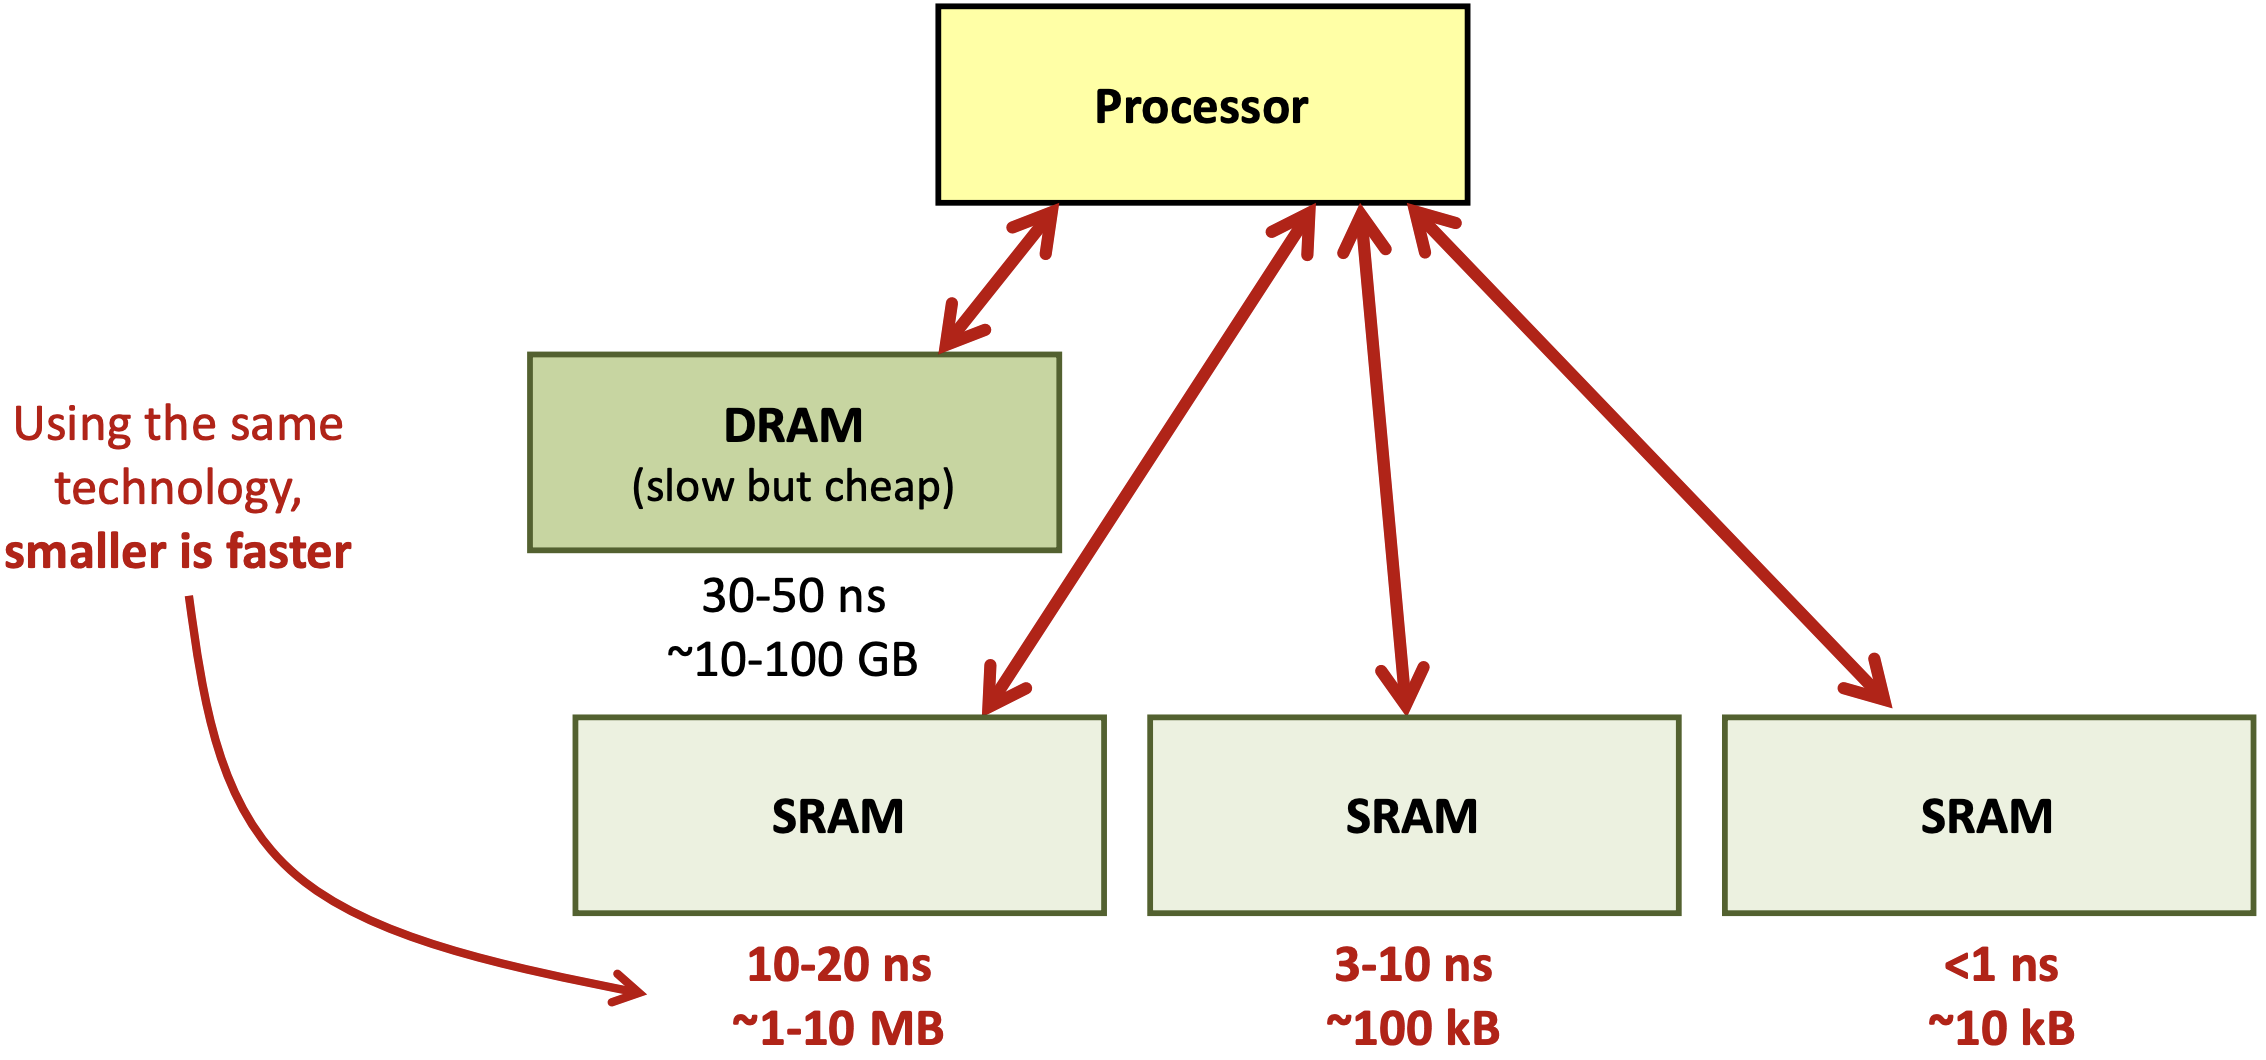
\includegraphics[width=0.65\textwidth]{chapters/chapter3a/images/hierarchy.png}
\end{center}
\begin{itemize}
    \item \textbf{DRAM (Dynamic Random Access Memory):}
    \begin{itemize}
        \item \textit{Characteristics:} DRAM is slow but cost-effective.
        \item \textit{Access Time:} Typically between 30 and 50 nanoseconds.
        \item \textit{Capacity:} Provides a large storage size, ranging from 10 GB to 100 GB.
    \end{itemize}
    
    \item \textbf{SRAM (Static Random Access Memory):}
    \begin{itemize}
        \item \textit{Characteristics:} SRAM is fast but expensive.
        \item \textit{Access Time:} Less than 1 nanosecond.
        \item \textit{Capacity:} Offers smaller storage sizes, around 10 KB.
    \end{itemize}
\end{itemize}

\textbf{Objective:} The goal is to leverage the advantages of both DRAM and SRAM to achieve an efficient memory system, combining the speed of SRAM with the cost-effectiveness and capacity of DRAM.

\begin{center}
    \textit{Can we get the best of both worlds?}
\end{center}


\subsection{What Memory ot Use?}
Efficient memory usage is crucial for ensuring high performance in iterative computations, as seen in the following example:
\begin{cc}
i = 0;
sum = 0;
while (i < 1024) {
    sum = sum + a[i];
    i = i + 1;
}
\end{cc}
\begin{itemize}
    \item \textbf{Instruction locality:} Instructions corresponding to lines 3-5 in the loop are read repeatedly. These should reside in fast memory (e.g., caches) to minimize latency.
    \item \textbf{Variable access:} Frequently accessed variables like \texttt{i} and \texttt{sum} should be stored in fast memory, such as registers or cache, to reduce access time.
    \item \textbf{Prefetching:} To improve performance, future instructions and array elements (e.g., \texttt{a[i+1]}, \texttt{a[i+2]}, etc.) can be loaded into memory in advance using techniques like hardware or software prefetching.
\end{itemize}

\subsection{Spatial and Temporal Locality}
Two important criteria for deciding on data placement in memory are:

\paragraph{Temporal Locality} This refers to data that has been \textbf{used recently} and thus has a high likelihood of being reused. Examples include:
\begin{itemize}
    \item \textbf{Code:} loops, functions, etc.
    \item \textbf{Data:} local variables and data structures.
\end{itemize}

\paragraph{Spatial Locality} This refers to data located \textbf{near other data currently in use}, which is likely to be accessed soon. Examples include:
\begin{itemize}
    \item \textbf{Code:} sequentially read instructions.
    \item \textbf{Data:} arrays and other contiguous structures.
\end{itemize}

\subsection{Placement Policy Design}

Our placement policy must satisfy two essential requirements:

\begin{itemize}
    \item \textbf{Invisible to the Programmer:}
    \begin{itemize}
        \item While it is possible to analyze data structures and program semantics to detect heavily used variables or arrays for placement decisions, this approach is only suitable in specific contexts (e.g., embedded systems).
        \item The goal is to alleviate the burden on programmers by introducing hardware mechanisms to manage placement transparently.
    \end{itemize}
    \item \textbf{Extremely Simple and Fast:}
    \begin{itemize}
        \item Placement decisions, when delegated to hardware, must be simple to ensure efficiency.
        \item The primary objective is to facilitate access to fast memory within nanoseconds or less, leaving little room for complex decision-making.
    \end{itemize}
\end{itemize}
\newpage
\section{Cache: The Idea}
Caching is a mechanism used to improve the performance of a computer system by storing frequently accessed data in a smaller, faster memory known as the cache. 
\begin{center}
    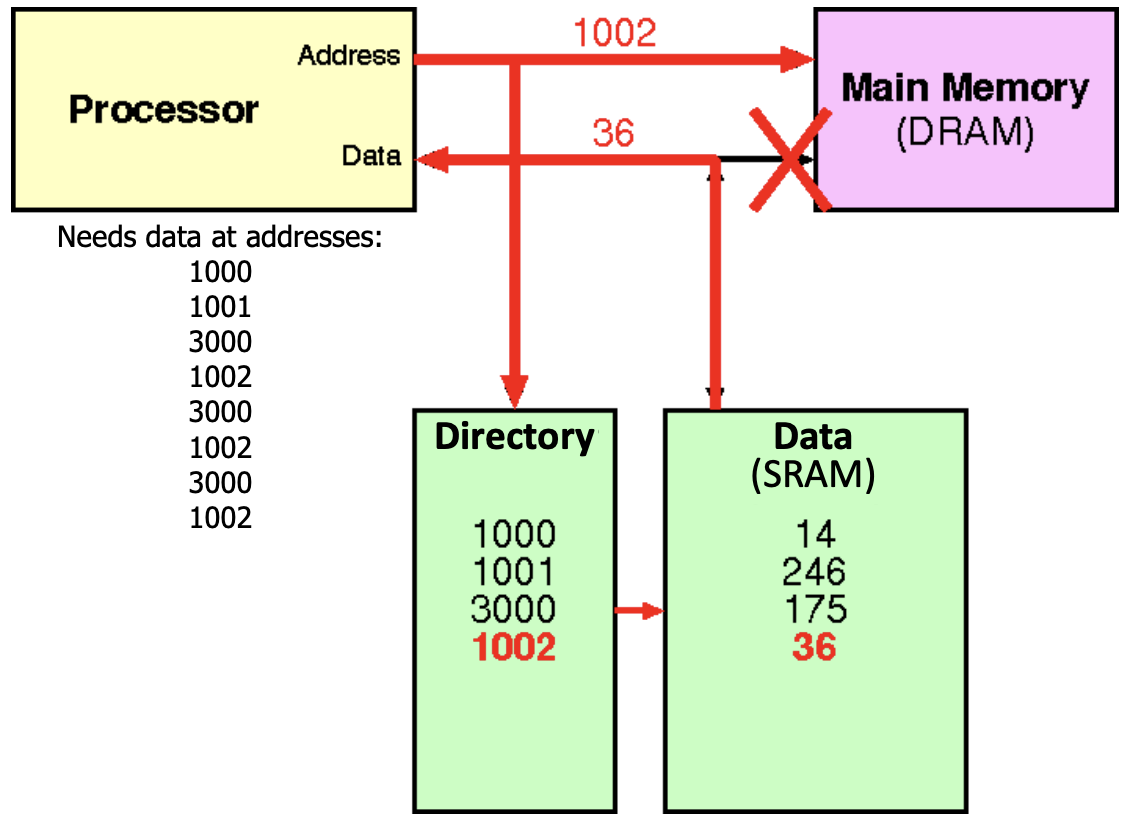
\includegraphics[width=0.45\textwidth]{chapters/chapter3a/images/cache.png}
\end{center}
\begin{itemize}
    \item[-] \textbf{Processor Request:} The processor requires data located at specific memory addresses, such as \texttt{1000}, \texttt{1001}, \texttt{3000}, and \texttt{1002}.
    \item[-] \textbf{Cache Directory and Data:} The cache maintains a directory that maps memory addresses to their corresponding data stored in the cache. For example, the data for address \texttt{1002} is located in the cache with a value of \texttt{36}.
    \item[-] \textbf{Cache Hit:} If the requested address exists in the cache directory (e.g., \texttt{1002}), the processor retrieves the data directly from the cache. This is referred to as a \textit{cache hit}.
    \item[-] \textbf{Cache Miss:} If the requested address is not found in the cache, the data is fetched from the main memory (DRAM), stored in the cache, and then delivered to the processor.
    \item[-] \textbf{Performance Benefit:} By prioritizing access to the cache (SRAM), which is faster than main memory (DRAM), the system reduces latency and improves overall performance.
\end{itemize}


\subsection{Cache Memory: Directory and Tags}
Cache memory is not just about speed but also about efficient management of data. Two critical components of a cache system are the \textbf{Directory} and \textbf{Tags}, which play a vital role in ensuring data consistency and fast access.
\begin{center}
    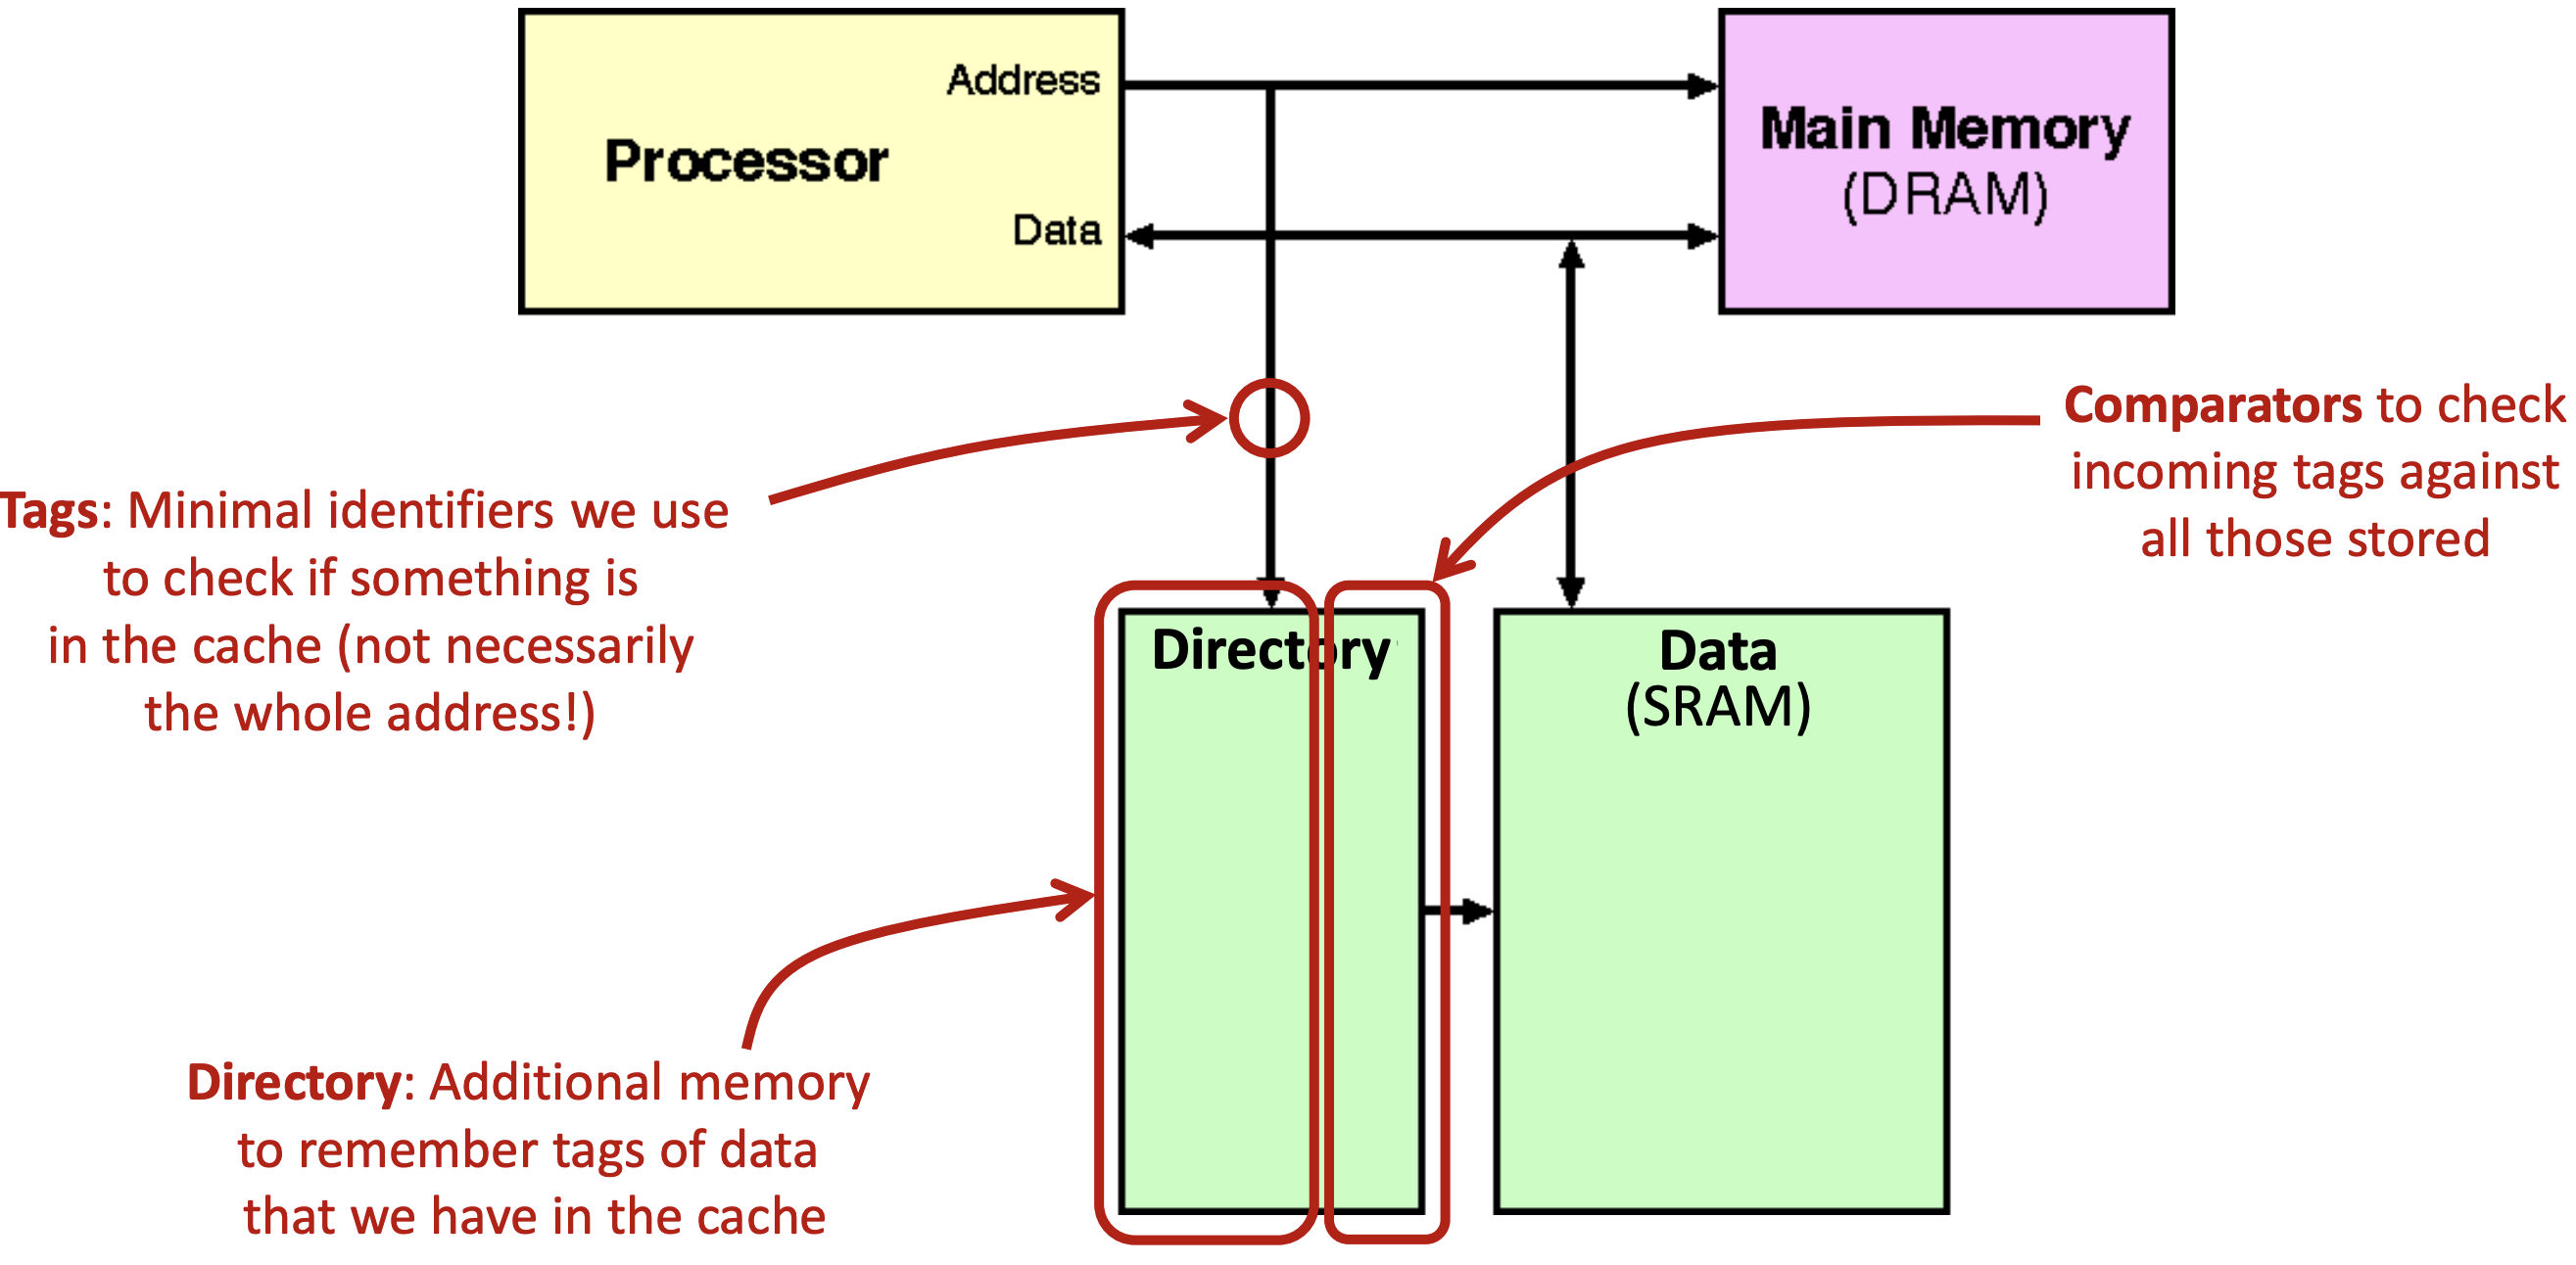
\includegraphics[width=0.65\textwidth]{chapters/chapter3a/images/cache2.png}
\end{center}
\begin{itemize}
    \item[-] \textbf{Tags:} Minimal identifiers used to determine if a specific data block is in the cache. These identifiers are typically smaller than the full memory address, optimizing comparison speed and storage requirements.
    \item[-] \textbf{Directory:} A dedicated memory structure that stores the tags of data currently present in the cache. This allows for efficient lookups and ensures the correct data is retrieved.
    \item[-] \textbf{Comparators:} Hardware elements that compare incoming tags against those stored in the directory. They enable quick validation of cache hits or misses.
\end{itemize}

\subsection{Cache Hits and Misses}
A \textbf{cache} is a form of storage that \textit{automatically} leverages the \textbf{locality of accesses} to improve performance. The concept has been widely adopted beyond processors, and examples include:

\begin{itemize}
    \item[-] Web browsers caching frequently accessed data.
    \item[-] Network routers caching routing information.
    \item[-] DNS servers caching frequent domain names.
    \item[-] Databases caching queries.
\end{itemize}

When the required data is found in the cache, it is called a \textbf{Hit}. Conversely, if the data is not found, it is termed a \textbf{Miss}.

The \textbf{Hit Rate} (or \textbf{Miss Rate}) is defined as the ratio of hits (or misses) to the total number of accesses.


\subsection{Fully-Associative Cache}

A fully-associative cache is a type of cache memory that allows any block of main memory to be stored in any cache line. 

\begin{center}
    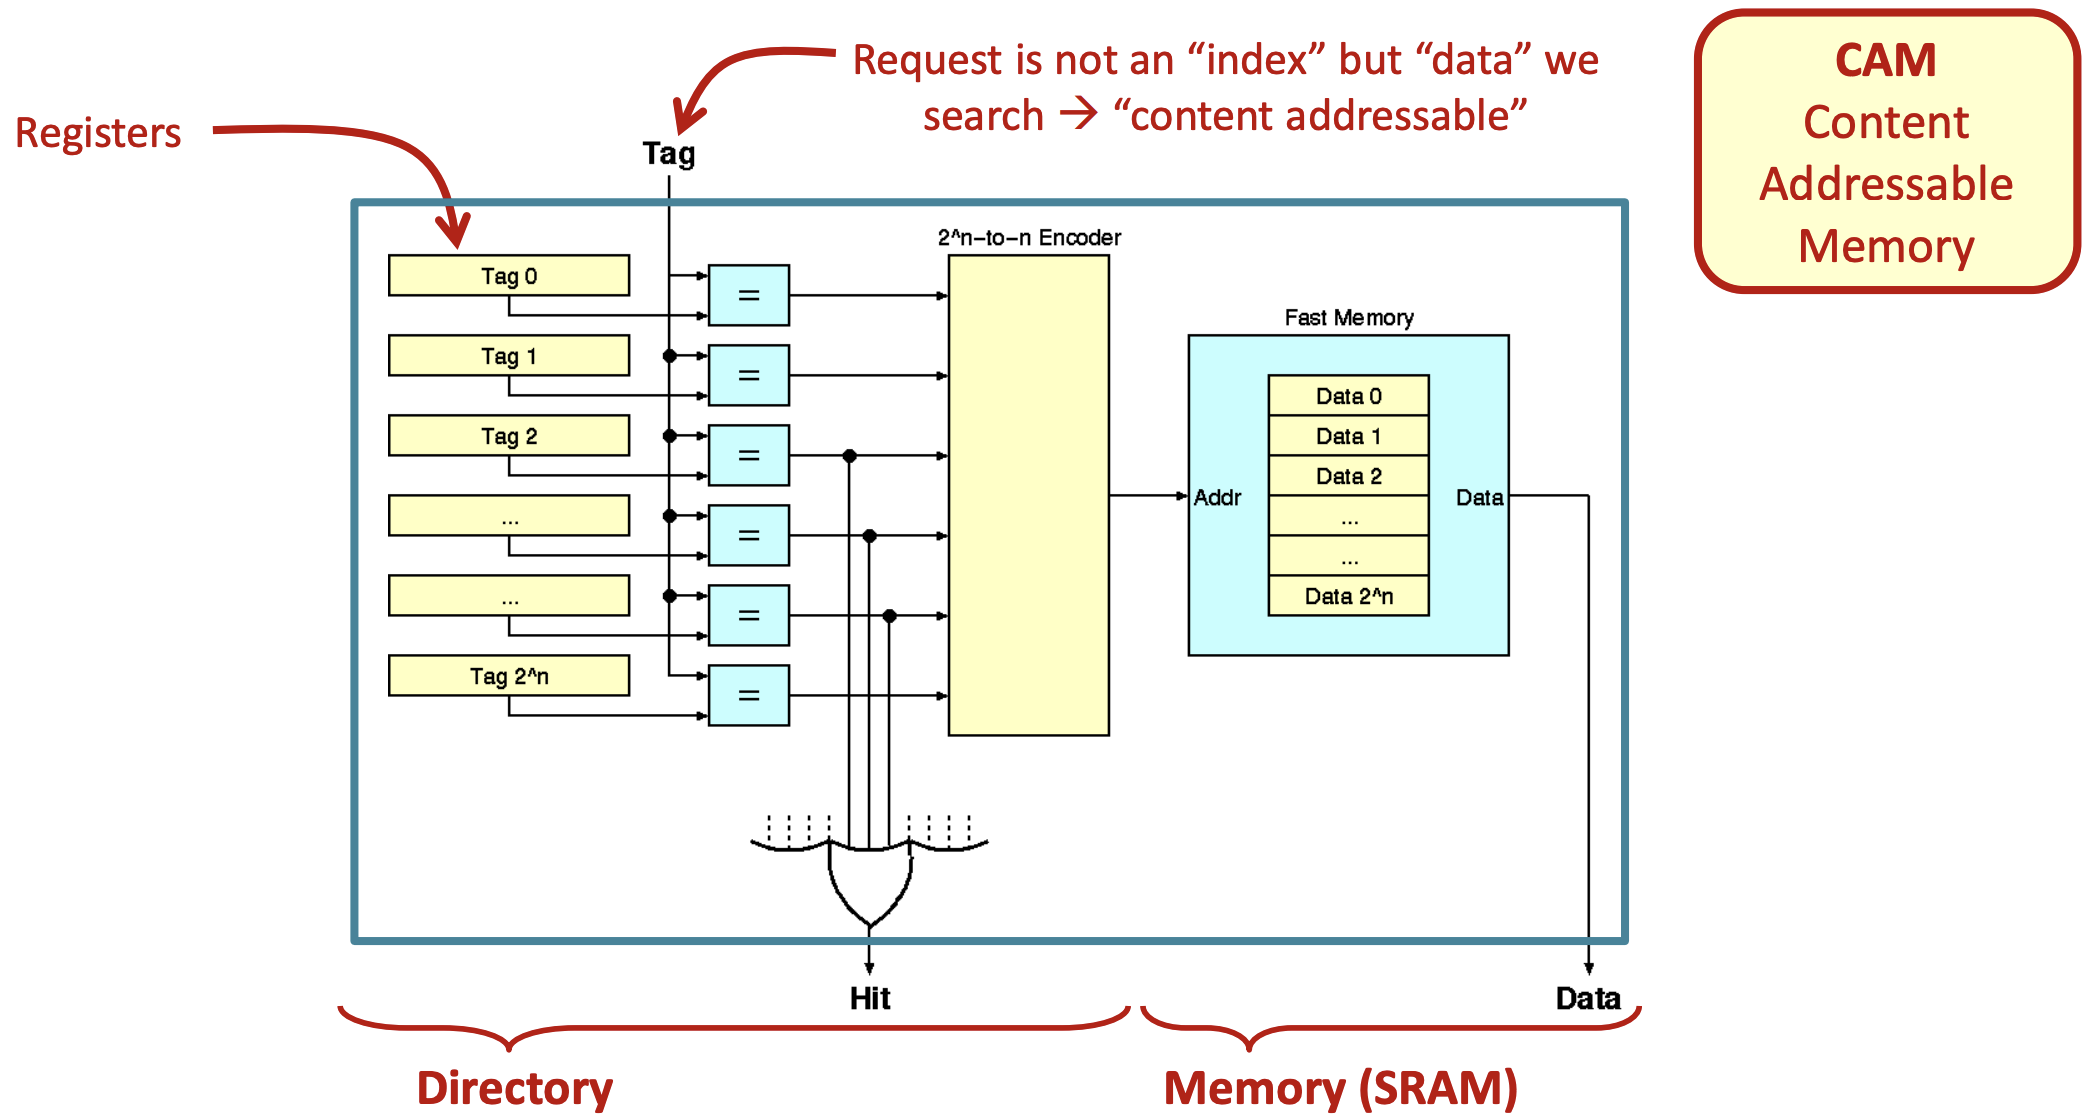
\includegraphics[width=0.75\textwidth]{chapters/chapter3a/images/cache3.png}
\end{center}
\subsubsection*{Key Components}
\begin{enumerate}
    \item \textbf{Directory (Tag Array):} Each entry in the tag array (referred to as "Tags") stores metadata about the cached blocks. Tags uniquely identify the memory block stored in each cache line.
    \item \textbf{Content Addressable Memory (CAM):} To find a specific block in the cache, the requested address is compared simultaneously with all stored tags. This parallel comparison is achieved using CAM, which enables \textit{content-based addressing}.
    \item \textbf{Comparison Logic:} The CAM outputs a signal indicating whether the requested tag matches any of the stored tags. This determines a \textit{hit} or \textit{miss}.
    \item \textbf{Fast Memory (SRAM):} This stores the actual data blocks associated with each tag. When a hit occurs, the data corresponding to the matched tag is retrieved from this memory.
    \item \textbf{Encoder:} If a match (hit) is found, the encoder selects the appropriate line from the data memory to access the requested data.
\end{enumerate}

\subsubsection*{How It Works}
\begin{enumerate}
    \item A memory access request is initiated with an address containing the desired data's \textit{tag}.
    \item The tag is compared in parallel against all tags stored in the directory using CAM.
    \item If a match is found, a \textit{hit} is signaled, and the corresponding data is retrieved from the fast memory using the encoder. If no match is found, a \textit{miss} occurs, and the block is fetched from main memory.
    \item The requested data is returned to the processor.
\end{enumerate}

\subsection{Fully-Associative Cache}

In a \textit{fully-associative cache}, any block of memory can be stored in any cache line. This flexibility removes the need for a specific mapping between memory blocks and cache lines, allowing for maximum utilization of cache space. 

\begin{center}
    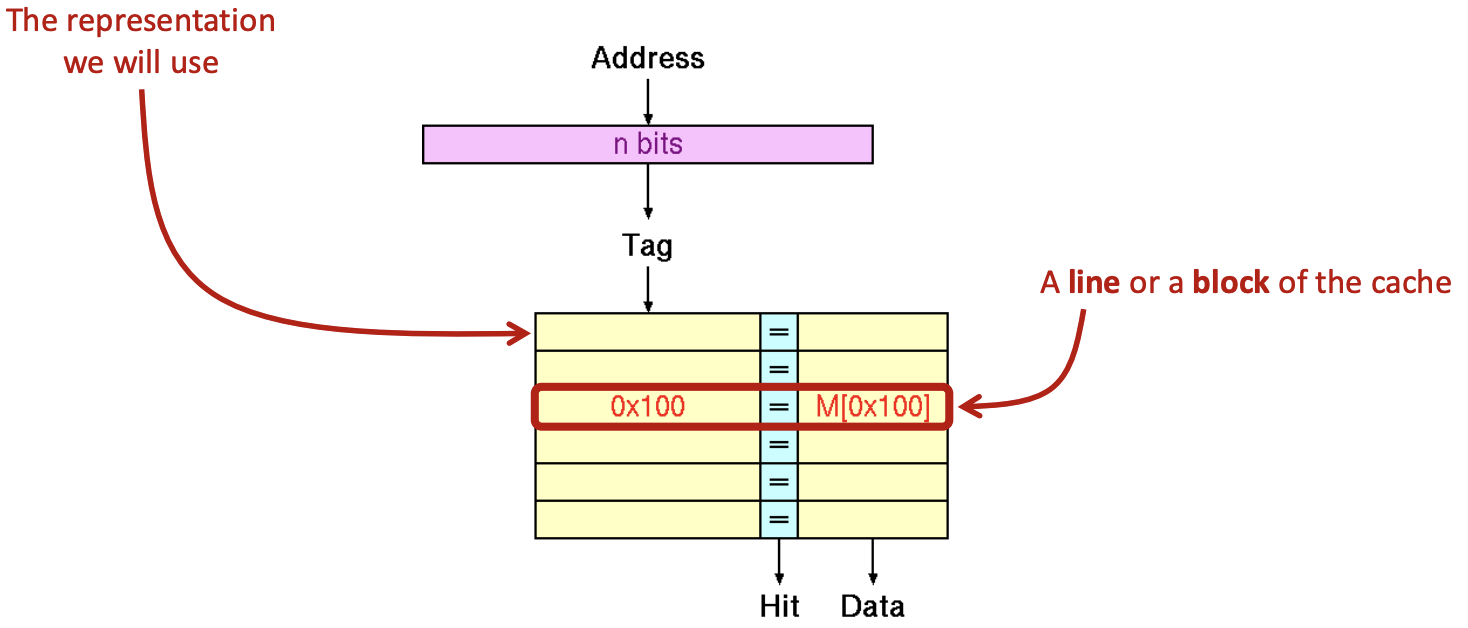
\includegraphics[width=0.65\textwidth]{chapters/chapter3a/images/cache4.png}
\end{center}
\begin{itemize}
    \item[-] \textbf{Address Representation:} The memory address is represented using $n$ bits. Each address can be divided into a \textit{tag} and an optional \textit{block offset} (if the cache stores data in blocks).
    \item[-] \textbf{Cache Lines:} Each line (or block) of the cache contains:
    \begin{enumerate}
        \item The \textit{tag} to identify the memory block stored in that line.
        \item The actual \textit{data} fetched from memory.
    \end{enumerate}
\end{itemize}

\section{Cache and Cache Controller}
The cache and cache controller system serves as an intermediary between the processor and the main memory to enhance the overall performance of memory access. Below is an explanation of each component in the system:
\begin{center}
    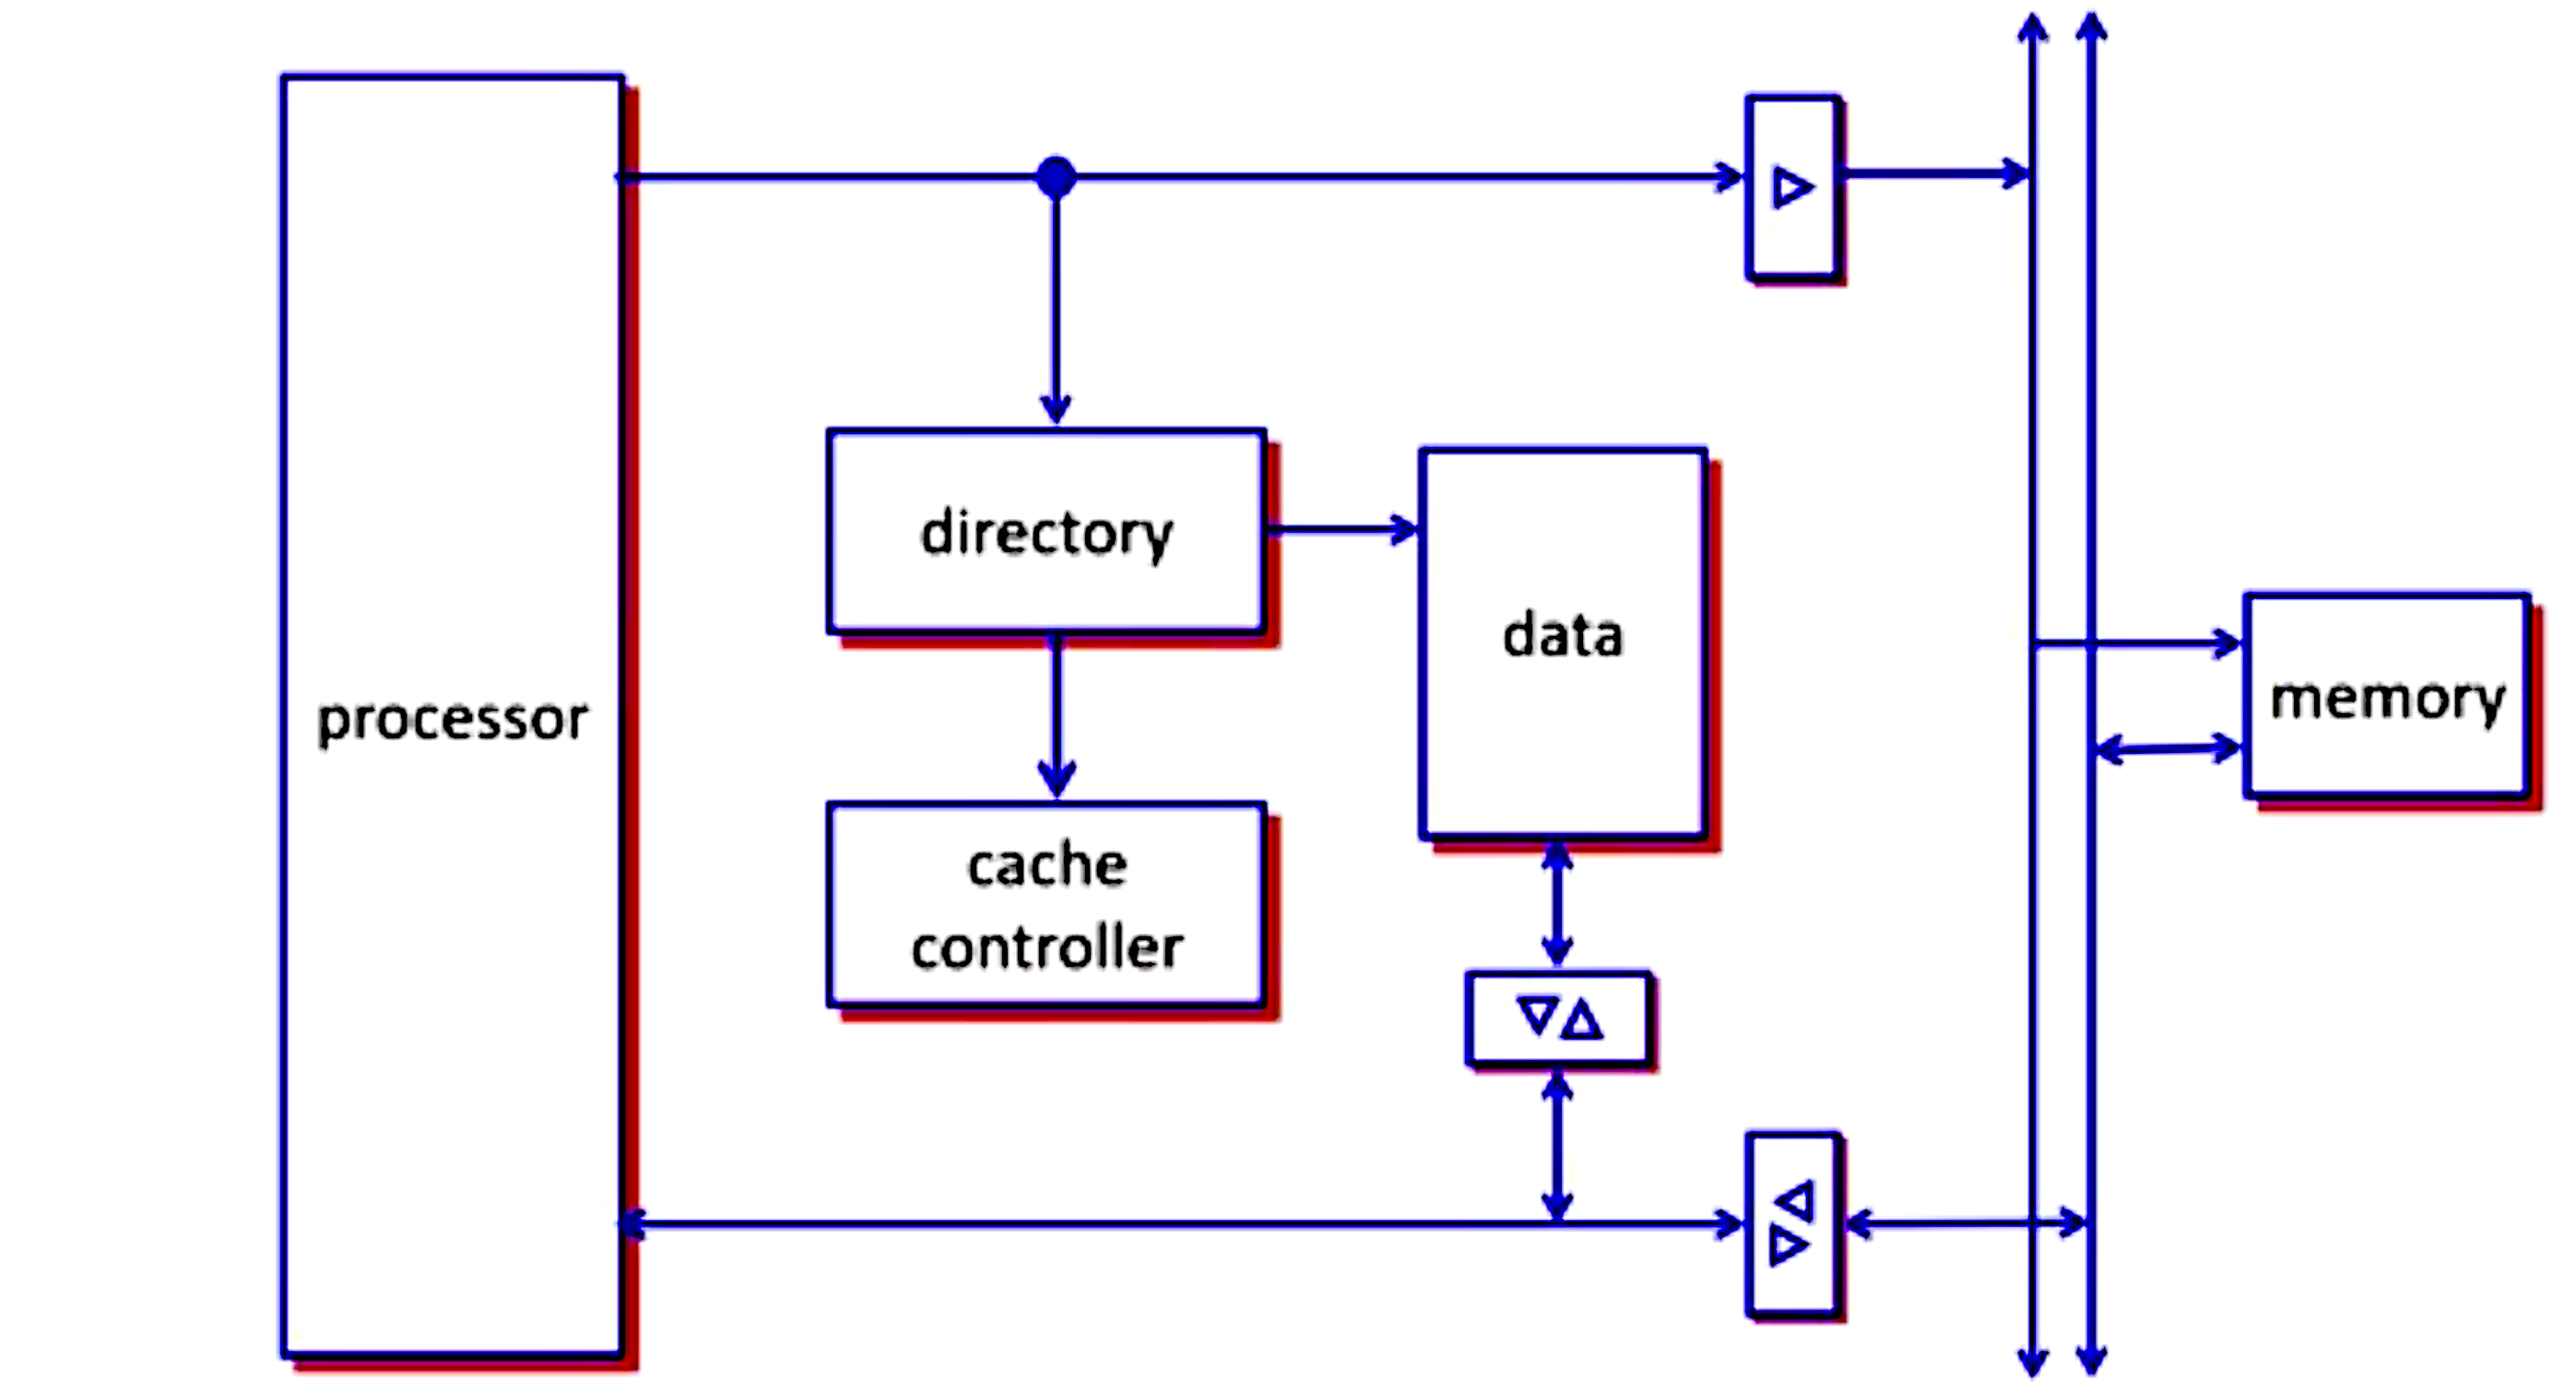
\includegraphics[width=0.55\textwidth]{chapters/chapter3a/images/cache_rep.png}
\end{center}

\begin{itemize}
    \item \textbf{Processor:} The central processing unit (CPU) that executes instructions and requests data from the memory hierarchy.

    \item \textbf{Directory:} A component that tracks the mapping of cached data to memory addresses. It determines whether a requested data item is present in the cache (cache hit) or not (cache miss).

    \item \textbf{Cache Controller:} This module manages the operation of the cache. It controls data flow between the directory, cache memory (data), and main memory. It ensures coherency and consistency of data when multiple memory requests occur.

    \item \textbf{Data:} The actual memory space within the cache that stores copies of frequently accessed data from main memory.

    \item \textbf{Main Memory:} The primary storage location that holds all data and instructions required by the processor. It communicates with the cache when the required data is not found in the cache (cache miss).

    \item \textbf{Bidirectional Arrows:} Indicate the flow of data between components. Data can flow from the processor to the cache, from the cache to the main memory, and vice versa.

    \item \textbf{Control Signals:} Represented as small triangular symbols, these signals are responsible for controlling the flow of data and ensuring synchronization between components.
\end{itemize}

\subsection{Cache Hit}
A \textit{cache hit} occurs when the processor requests data that is present in the cache. This scenario significantly improves performance by reducing the latency associated with memory access.
\begin{center}
    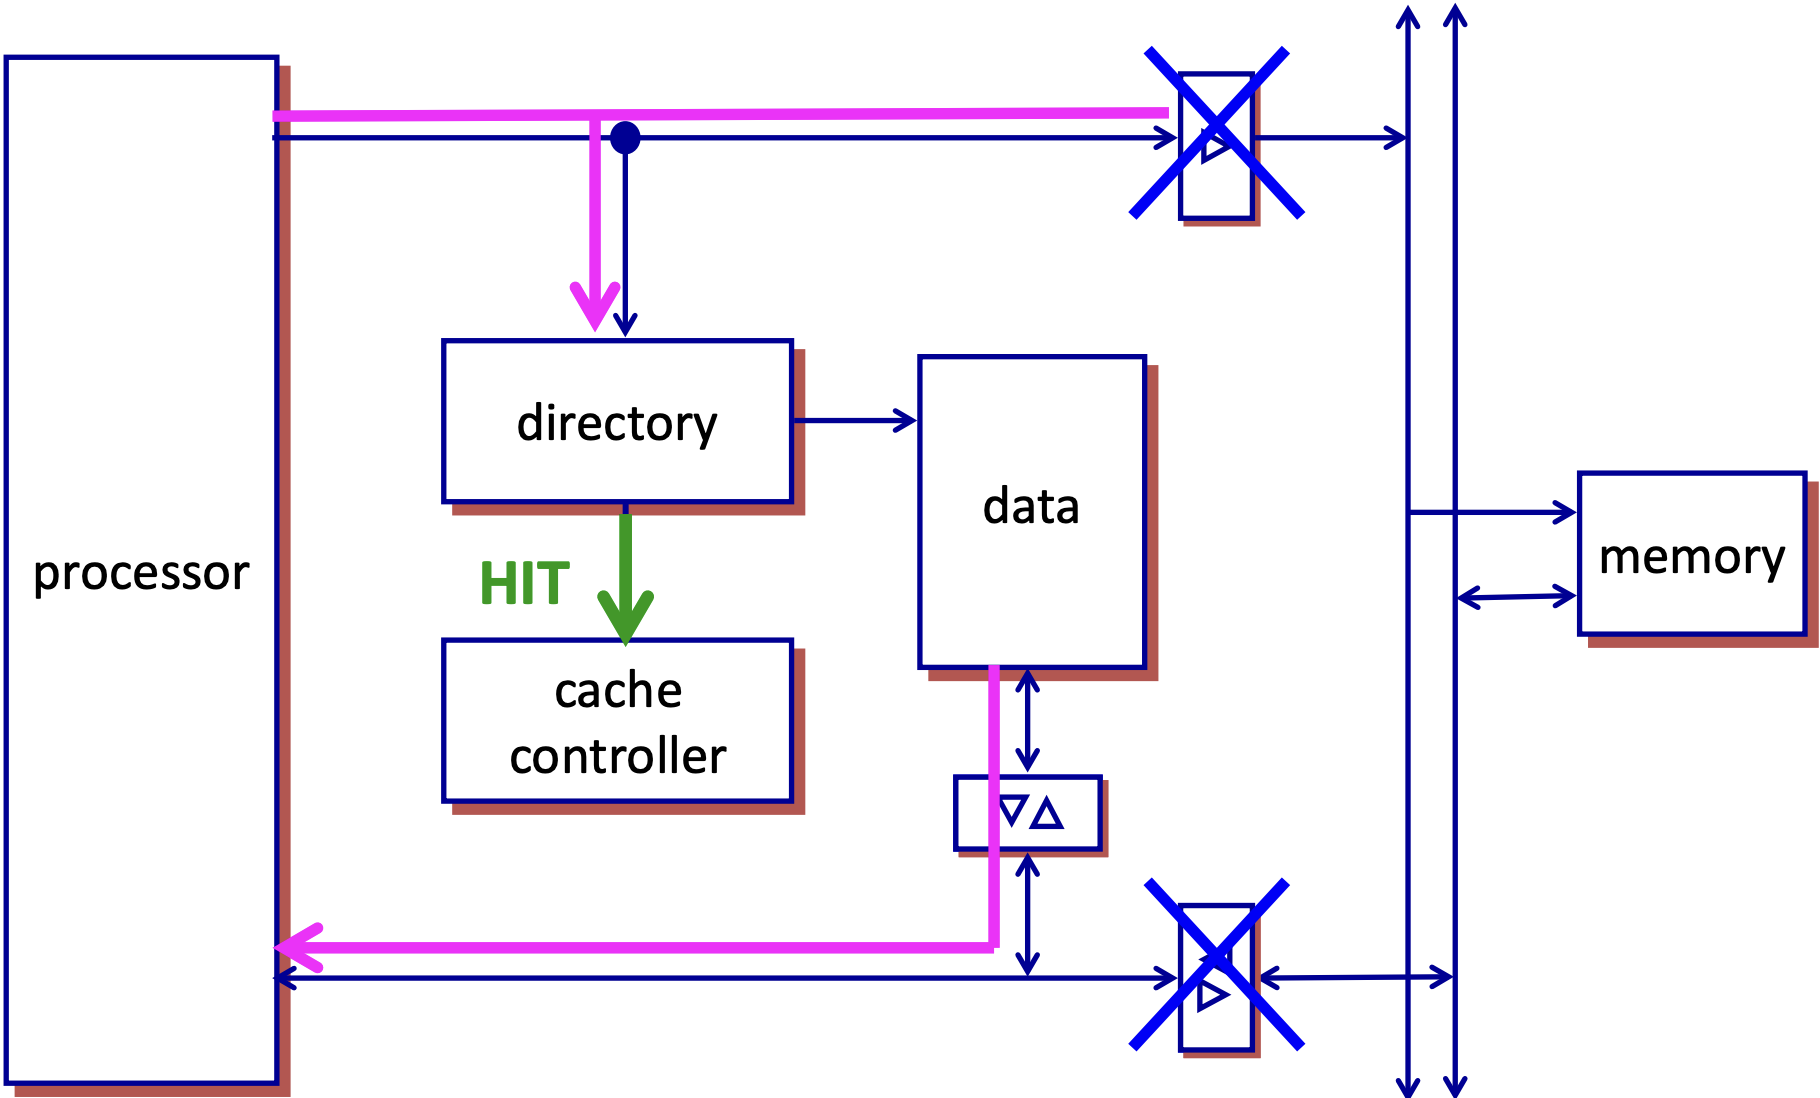
\includegraphics[width=0.55\textwidth]{chapters/chapter3a/images/hit.png}
\end{center}
\begin{enumerate}
    \item The processor sends a request for a specific data item.
    \item The \textit{directory} checks whether the requested data is available in the cache.
    \item If a match is found, a \textit{hit} is registered, and the \textit{cache controller} retrieves the data from the cache.
    \item The requested data is then sent directly back to the processor without accessing the main memory, as indicated by the absence of memory interaction in this scenario.
\end{enumerate}

\subsection{Cache Miss}
A cache miss occurs when the requested data is not present in the cache, requiring retrieval from the main memory. 
\begin{center}
    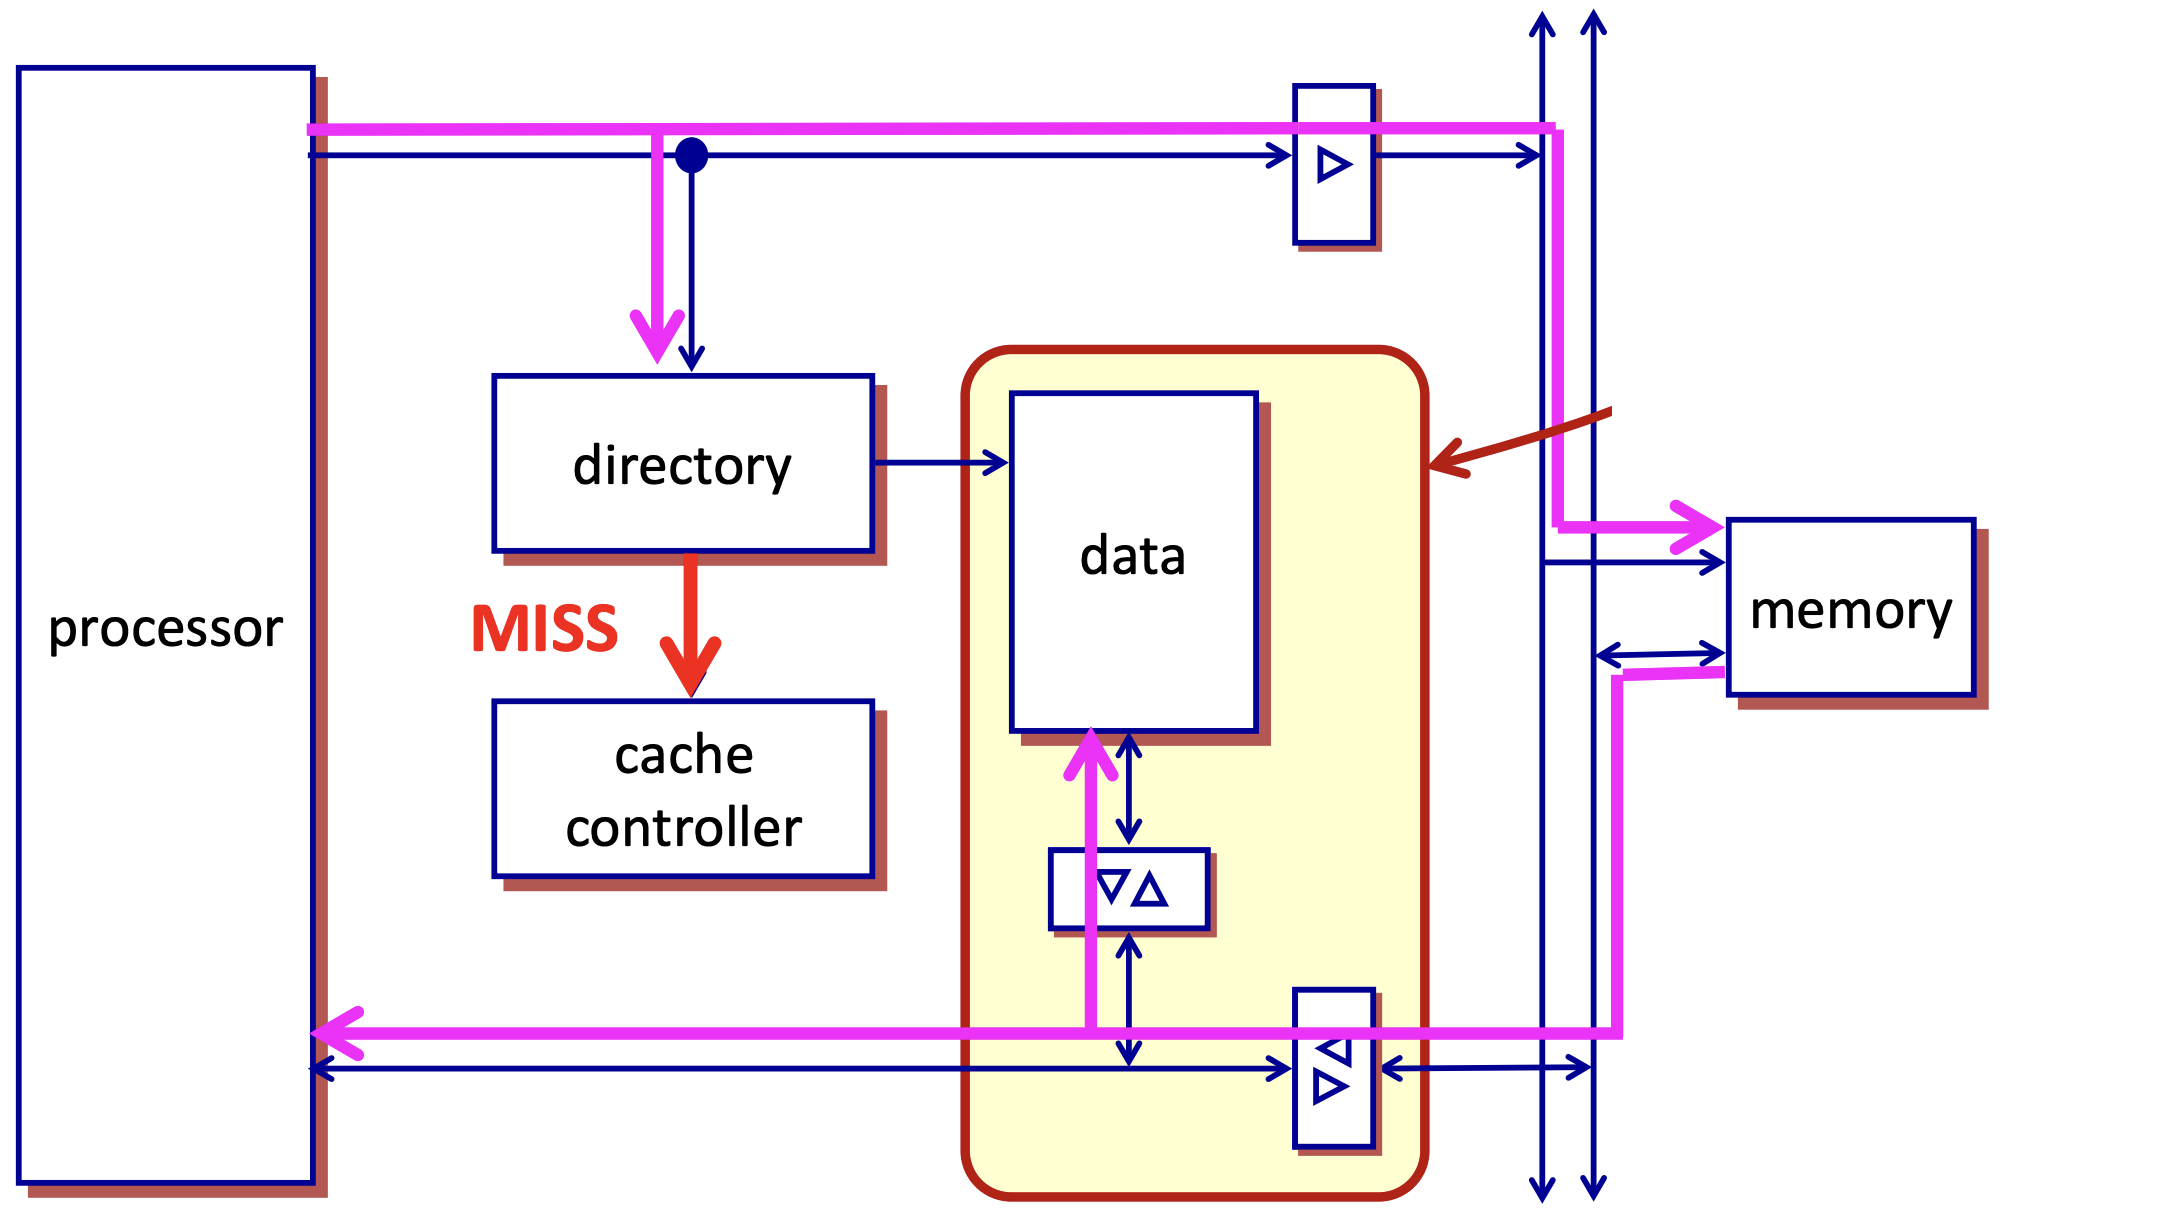
\includegraphics[width=0.55\textwidth]{chapters/chapter3a/images/miss.png}
\end{center}
\begin{enumerate}
    \item \textbf{Processor Request:} The processor issues a request for data. The request is forwarded to the cache directory.
    \item \textbf{Directory Check:} The directory checks whether the requested data is present in the cache. If the data is not found, a \textit{cache miss} is detected, and the directory informs the cache controller.
    \item \textbf{Cache Controller:} Upon detecting a cache miss, the cache controller initiates a fetch operation from the main memory. It ensures that the requested data is retrieved and forwarded to the processor.
    \item \textbf{Memory Access:} The cache controller sends a request to the main memory for the missing data. The memory responds by transferring the data back to the cache.
    \item \textbf{Cache Update:} The retrieved data is stored in the cache for future use. The directory is updated to reflect the new data location in the cache.
    \item \textbf{Processor Response:} Once the data is available in the cache, it is sent to the processor to fulfill the original request.
\end{enumerate}

\section{What if the Cache is Full?}
When the cache is full, adding new data requires the eviction of existing data to make space. This process is governed by a \textbf{cache replacement policy}. 
\begin{center}
    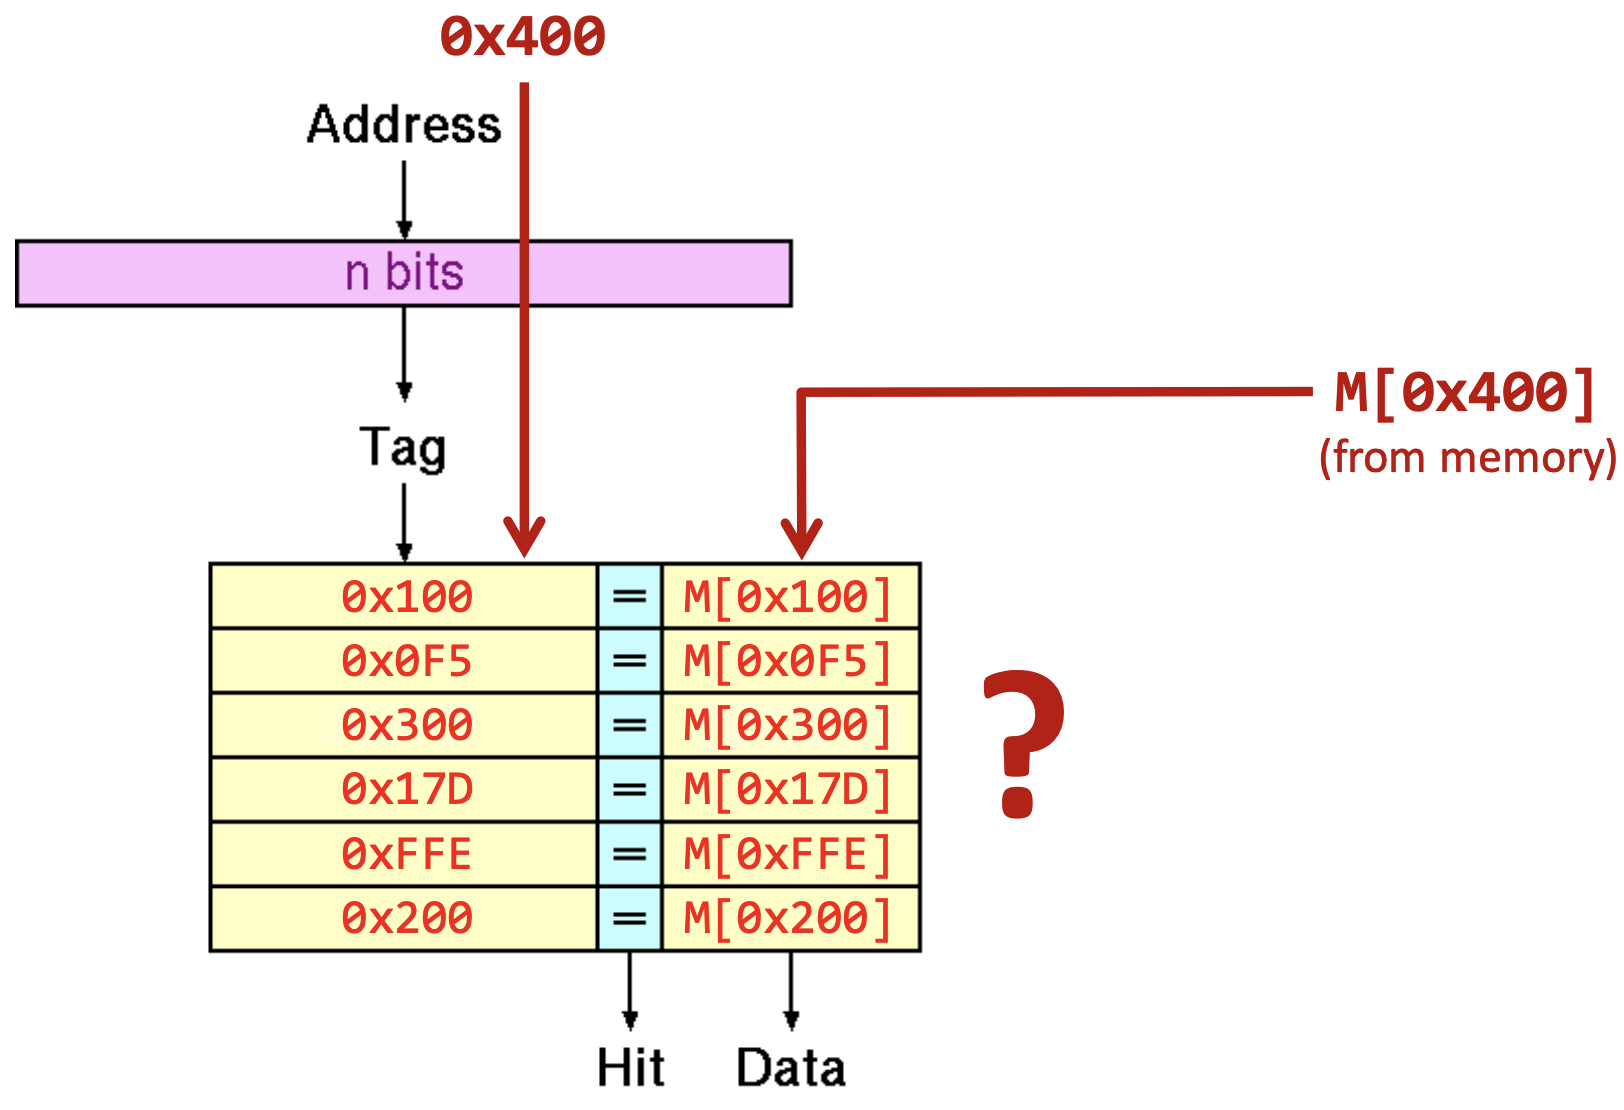
\includegraphics[width=0.45\textwidth]{chapters/chapter3a/images/full.png}
\end{center}
\subsection{Eviction Policies}
Various eviction policies determine which data to remove when the cache reaches its capacity limit. Common policies include:

- \textbf{Least Recently Used (LRU):} 
\begin{itemize}
\item Replaces the data that has been unused for the longest time.
\end{itemize}

- \textbf{First-In-First-Out (FIFO):} 
\begin{itemize}
\item Evicts the oldest data in the cache, based on the order of entry.
\end{itemize}

- \textbf{Random Replacement:} 
\begin{itemize}
\item Selects a cache line at random for eviction, regardless of usage or age.
\end{itemize}

- \textbf{Approximate Schemes:} 
\begin{itemize}
\item Use heuristics or approximations to determine eviction, balancing simplicity and performance.
\end{itemize}

Choosing the appropriate eviction policy depends on the application's requirements, balancing factors like speed, complexity, and data access patterns.
\newpage
\subsection{Only Exploiting Temporal Locality}
Temporal locality refers to the principle that data recently accessed is likely to be accessed again in the near future. In this approach:
\begin{center}
    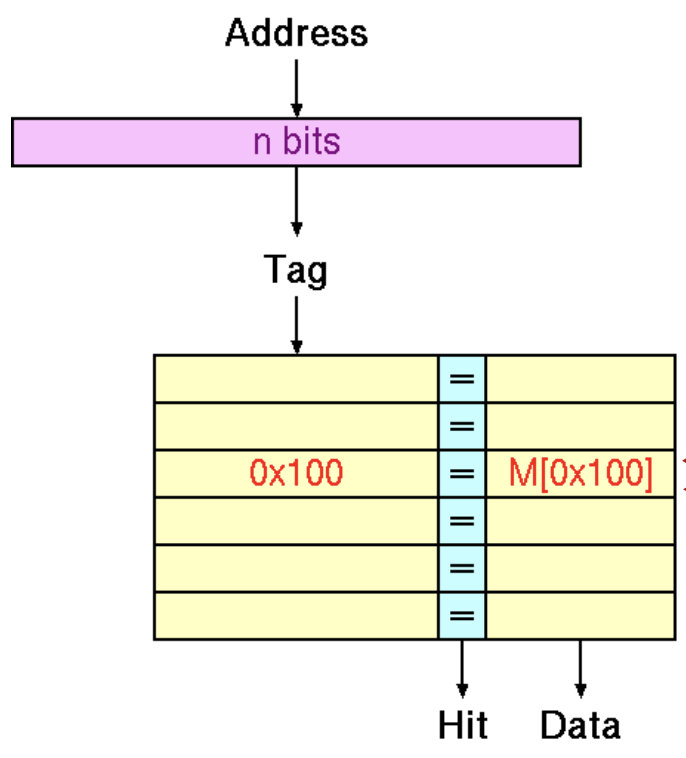
\includegraphics[width=0.25\textwidth]{chapters/chapter3a/images/temporal.png}
\end{center}
\begin{itemize}
    \item \textbf{Exclusive Data Fetching:} Only the specific data requested by the processor is fetched from the main memory into the cache, with the assumption that it will be reused soon.
    
    \item \textbf{Limitation:} This strategy does not account for \textit{spatial locality}, which predicts that data stored near the requested data is also likely to be accessed. For example:
    \begin{itemize}
        \item If the processor requests data at address \texttt{M[0x100]}, only this specific data is loaded into the cache.
        \item If the processor later requires data at \texttt{M[0x101]} (a neighboring address), it results in a cache miss since this data is not preloaded.
    \end{itemize}
    
    \item \textbf{Implication:} By focusing solely on temporal locality, the system may fail to optimize performance for workloads that benefit from spatial locality.
\end{itemize}
\subsection{Exploiting Spatial Locality}
Spatial locality refers to the tendency of a program to access data locations that are close to one another within a short period. To optimize memory performance, the concept of spatial locality involves fetching more data than just the requested word. This process is outlined below:
\begin{center}
    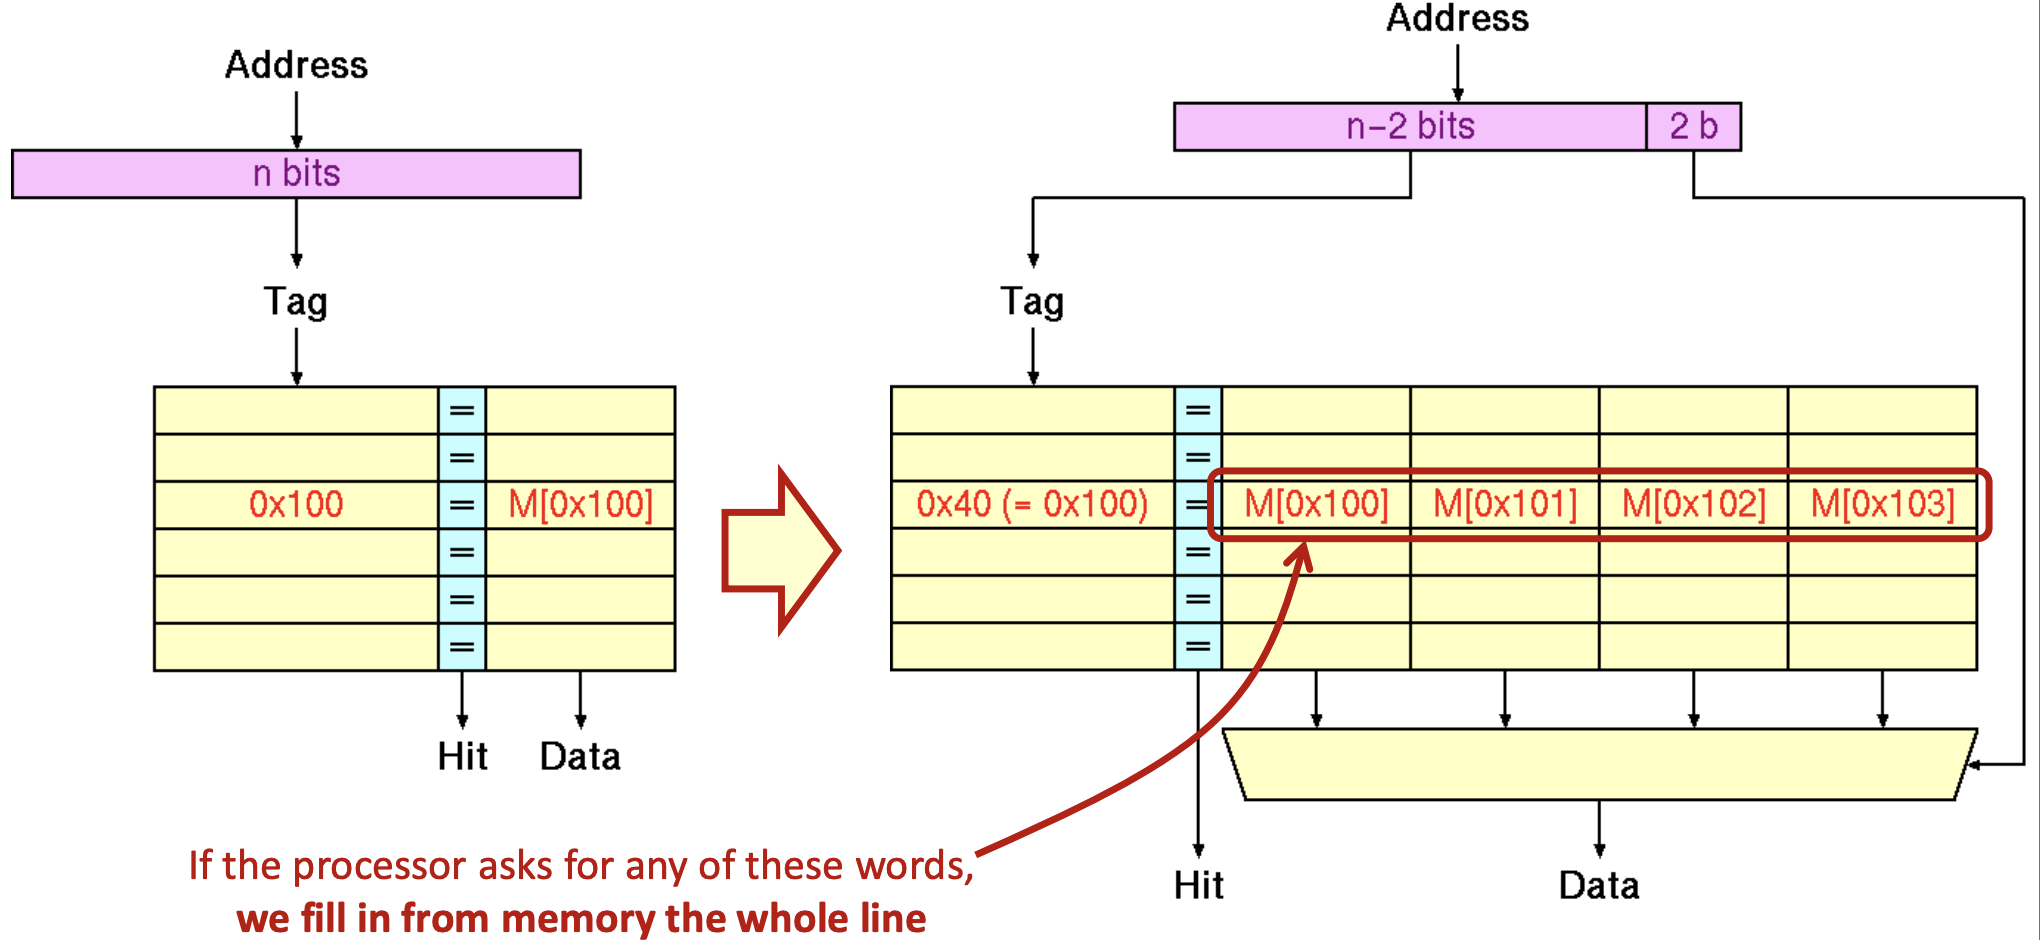
\includegraphics[width=0.65\textwidth]{chapters/chapter3a/images/spatial.png}
\end{center}
\begin{itemize}
    \item \textbf{Fetching Multiple Words:} When the processor requests data at a specific address (e.g., \texttt{M[0x100]}), the cache not only loads the requested word but also its neighboring words (e.g., \texttt{M[0x101]}, \texttt{M[0x102]}, and \texttt{M[0x103]}).
    \item \textbf{Cache Line:} The cache is structured in terms of lines, where each line contains multiple contiguous memory words. When a memory block is fetched, the entire line is populated in the cache.
    \item \textbf{Advantages:}
    \begin{itemize}
        \item Reduces the number of cache misses for sequential or nearby data accesses.
        \item Improves overall performance for workloads with high spatial locality.
    \end{itemize}
    \item \textbf{Example Scenario:} In the diagram:
    \begin{itemize}
        \item A request for \texttt{M[0x100]} results in the cache fetching an entire block containing \texttt{M[0x100]}, \texttt{M[0x101]}, \texttt{M[0x102]}, and \texttt{M[0x103]}.
        \item If the processor subsequently requests \texttt{M[0x101]}, it is already available in the cache, avoiding a cache miss.
    \end{itemize}
\end{itemize}

\subsection{Why Not This ?}
In a cache system, proper address matching and block selection are critical for accurate data retrieval. This subsection explores a specific scenario where matching the tag alone is insufficient and additional logic is required.
\begin{center}
    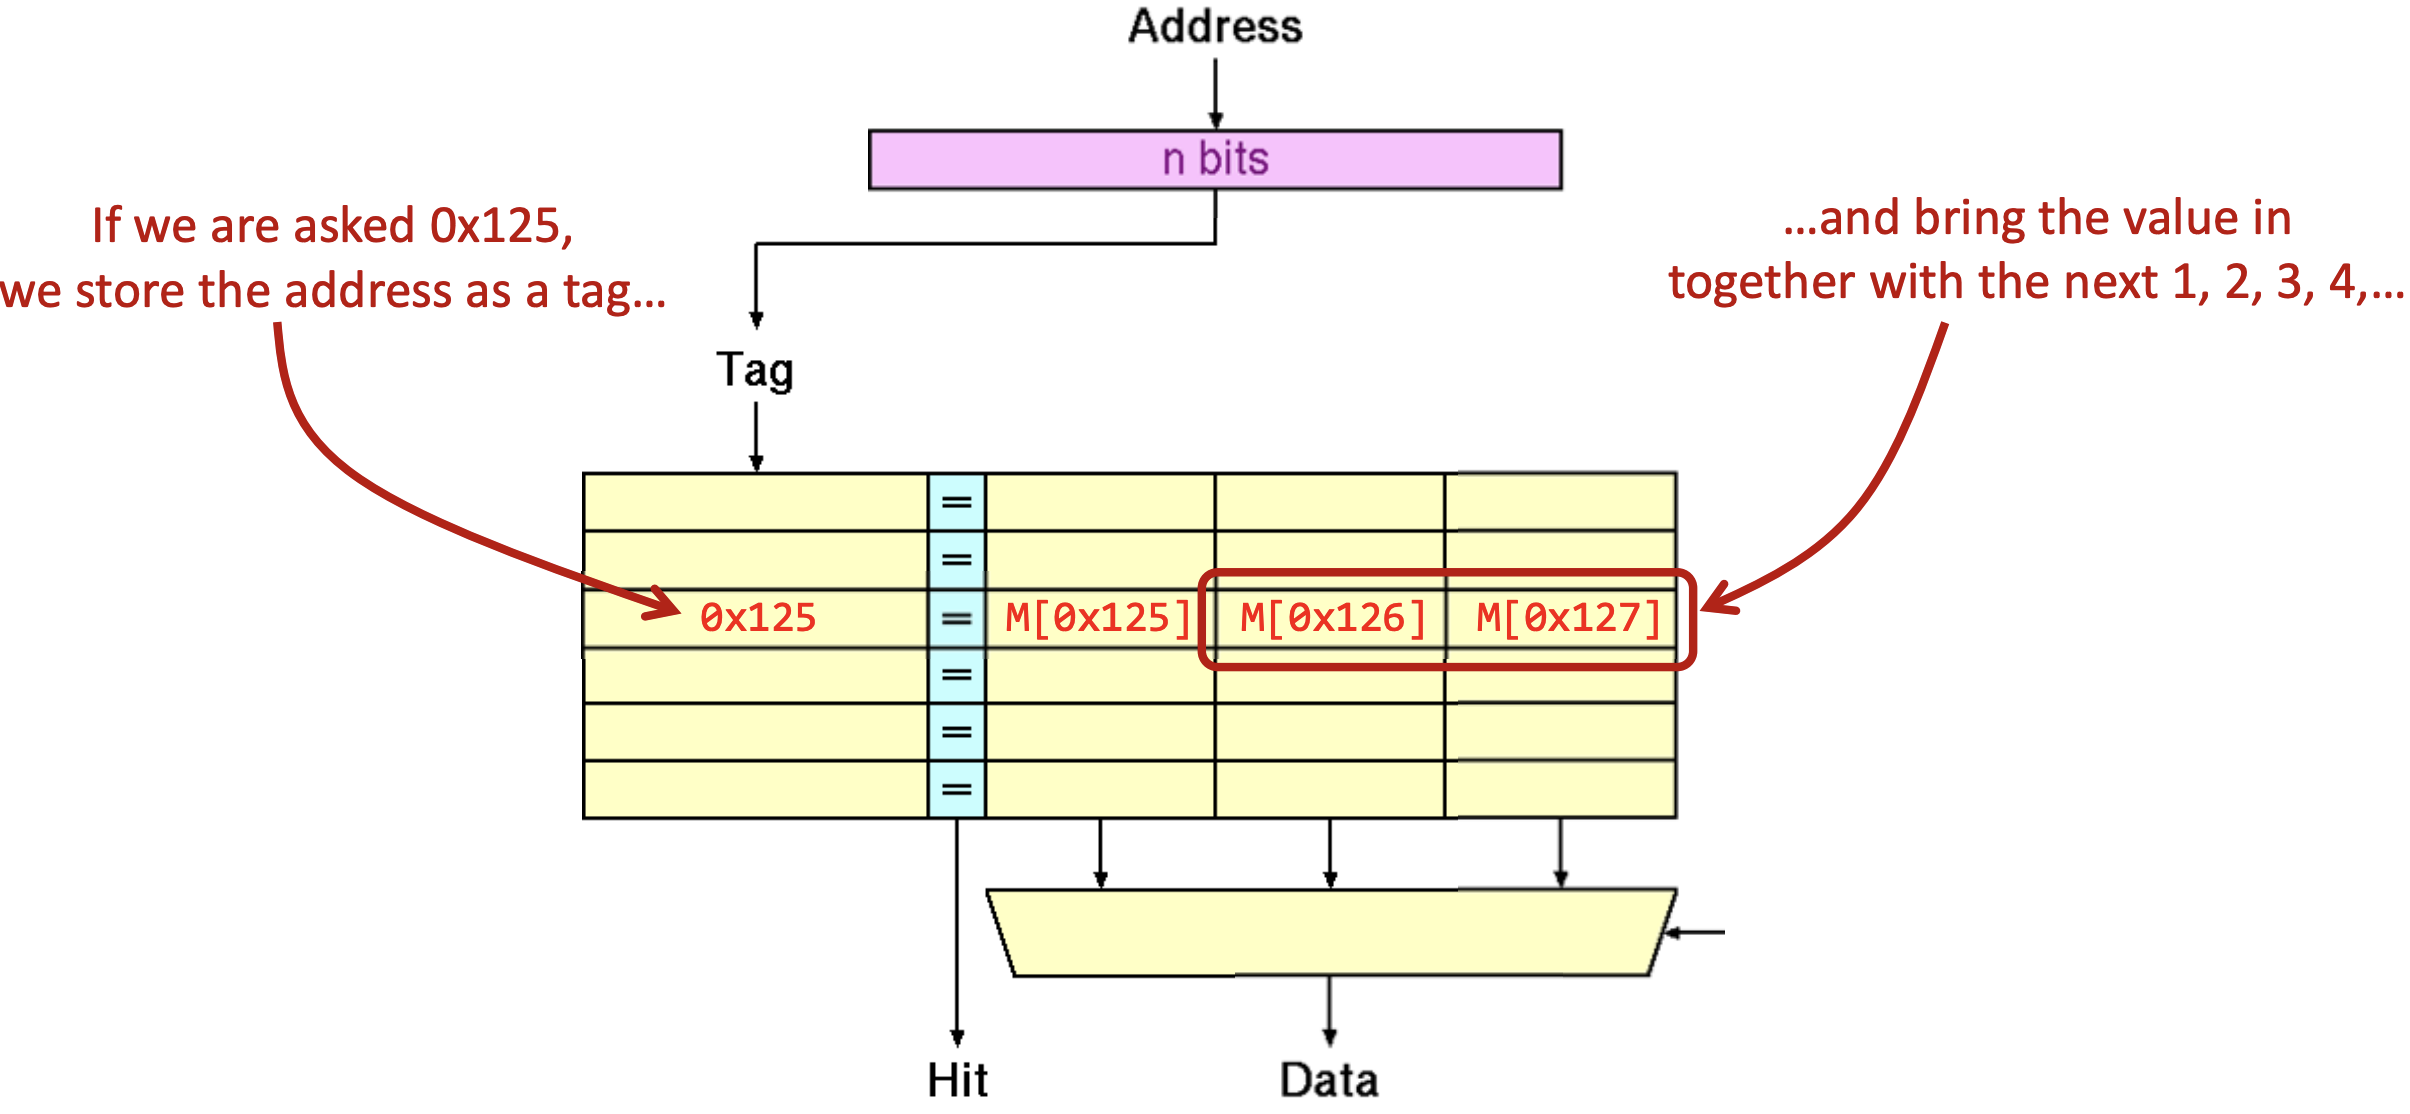
\includegraphics[width=0.75\textwidth]{chapters/chapter3a/images/notthis.png}
\end{center}
\begin{itemize}
    \item \textbf{Address and Tag Matching:} 
    \begin{itemize}
        \item The memory address is divided into a \textit{tag} and an \textit{offset}.
        \item The tag helps identify if the requested address corresponds to a block in the cache.
    \end{itemize}
    \item \textbf{Problem:} 
    \begin{itemize}
        \item If a requested address (e.g., \texttt{0x127}) is part of a cached block identified by the tag \texttt{0x125}, the tag comparison alone cannot directly confirm the presence of the requested word.
        \item The system must verify whether the requested address falls within the valid range of the block:\\
         \texttt{Tag $\leq$ Address $<$ Tag + Block Size}.
    \end{itemize}
\end{itemize}
\newpage
\subsection{Solution}
Efficient cache access relies on proper alignment and the use of power-of-2 elements per cache line.
-\textit{Personal Remark: The choice of a power of 2 is based on an absolute masterpiece that can be very useful, $A \% 2^n = A \& (2^n -1)$}
\begin{center}
    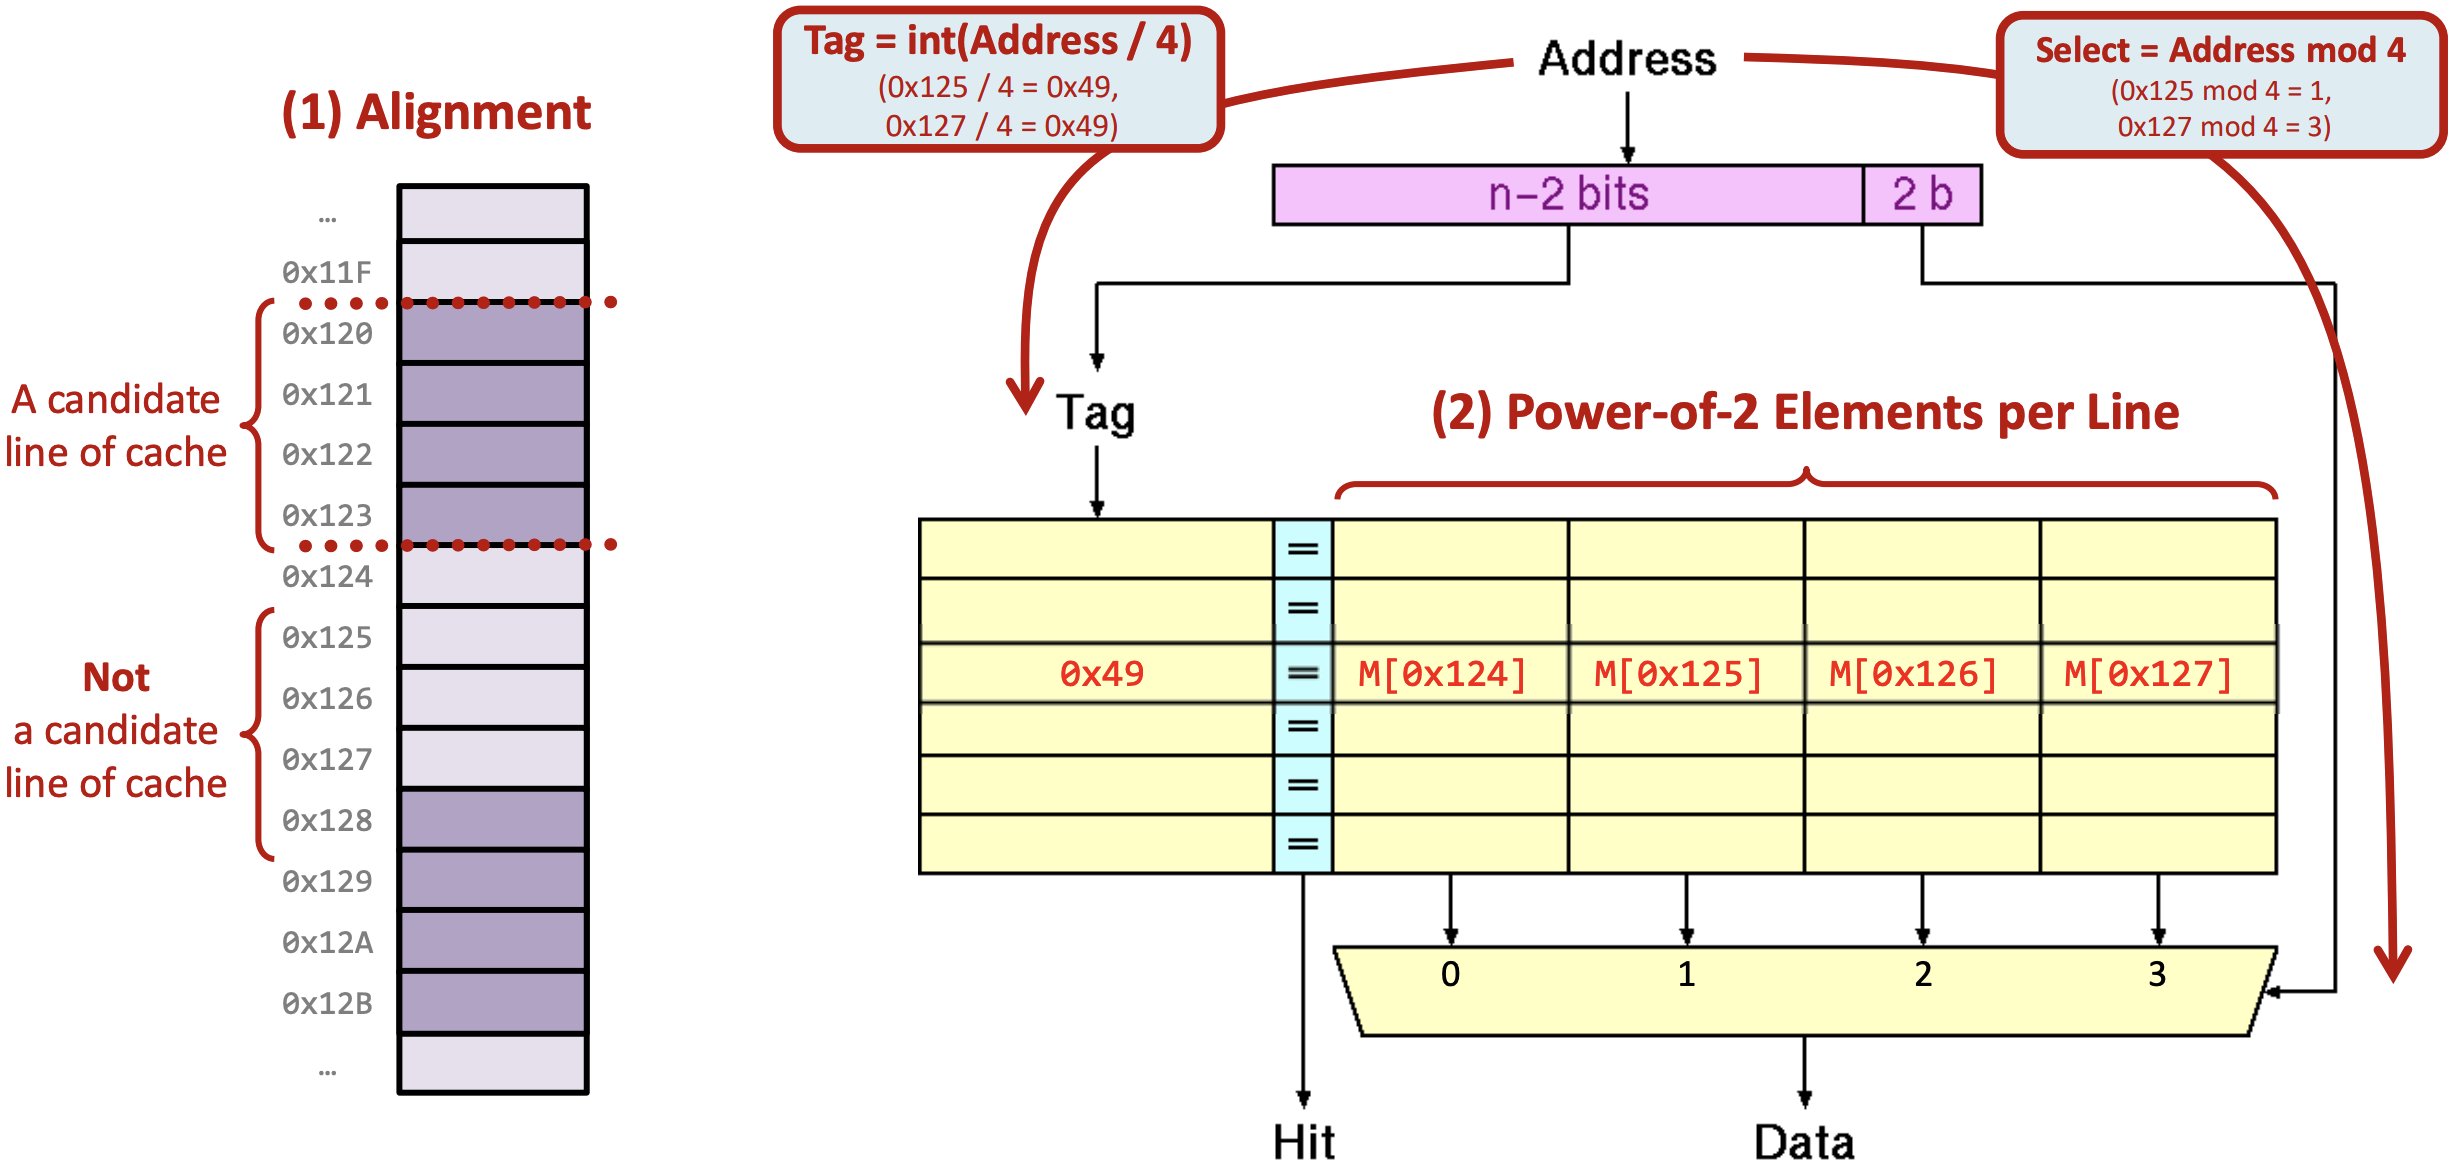
\includegraphics[width=0.75\textwidth]{chapters/chapter3a/images/solution.png}
\end{center}
\begin{itemize}
    \item \textbf{Alignment of Cache Lines:}
    \begin{itemize}
        \item Memory addresses are divided into fixed-sized cache lines, with alignment based on the size of the line.
        \item Only aligned addresses can serve as valid starting points for cache lines. For example:
        \begin{itemize}
            \item Address \texttt{0x124} is a valid starting point.
            \item Address \texttt{0x125} is not aligned and, therefore, cannot initiate a cache line.
        \end{itemize}
    \end{itemize}

    \item \textbf{Tag Calculation:}
    \begin{itemize}
        \item The tag is computed as \texttt{Tag = int(Address / Line Size)}.
        \item For example:
        \begin{itemize}
            \item \texttt{Tag(0x125) = int(0x125 / 4) = 0x49}.
            \item \texttt{Tag(0x127) = int(0x127 / 4) = 0x49}.
        \end{itemize}
    \end{itemize}

    \item \textbf{Power-of-2 Elements per Line:}
    \begin{itemize}
        \item Each cache line contains a power-of-2 number of elements (e.g., 4 elements per line).
        \item The specific word within the cache line is selected using the offset:
        \begin{itemize}
            \item \texttt{Select = Address mod Line Size}.
            \item Example: \texttt{0x125 mod 4 = 1} selects the second word.
        \end{itemize}
    \end{itemize}
\end{itemize}
\newpage
\subsection{Simplifying Cache Design}
Simplifying the cache design can reduce hardware complexity and improve performance.
\begin{center}
    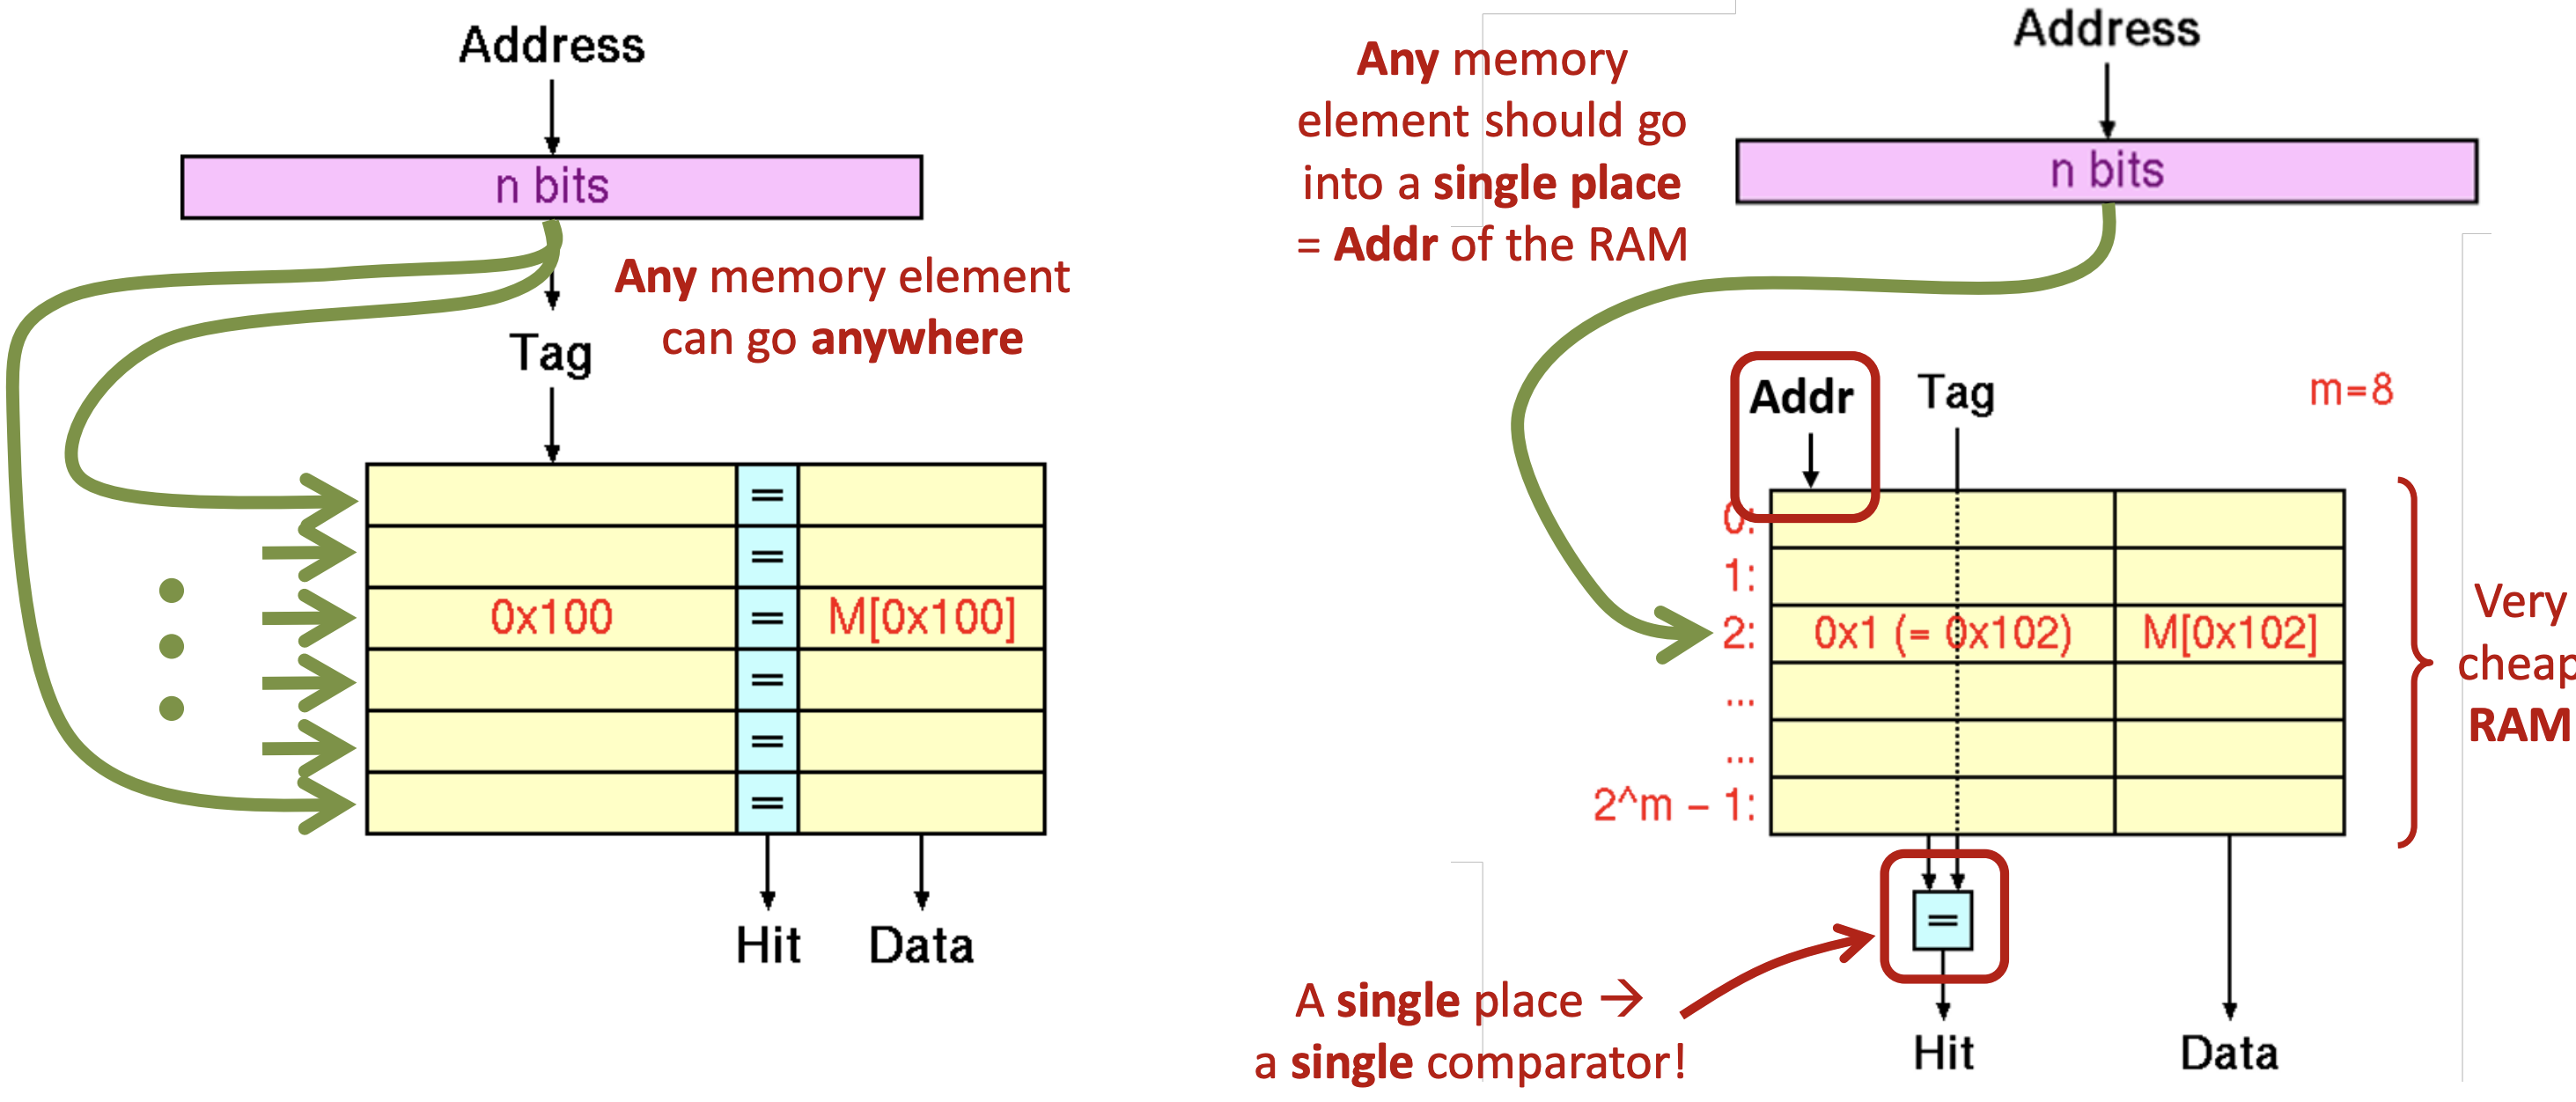
\includegraphics[width=0.65\textwidth]{chapters/chapter3a/images/simple.png}
\end{center}

\textbf{Current Approach:}
\begin{itemize}
    \item Memory elements can map to any cache line, requiring multiple comparators to check the tags across all lines.
    \item This increases hardware cost and complexity.
\end{itemize}

\textbf{Simplified Approach:}
\begin{itemize}
    \item Each memory element is mapped to a single, fixed cache location determined by its address.
    \item The cache uses the lower bits of the address to index into a specific line (\texttt{Addr} field).
    \item The \texttt{Tag} field contains the higher bits of the address to verify if the correct block is cached.
\end{itemize}

\section{Generating \texttt{Addr} and \texttt{Tag}}
The process of generating the \texttt{Addr} and \texttt{Tag} from a memory address ensures efficient mapping and lookup in the cache. The procedure involves splitting the address into two components:
\begin{center}
    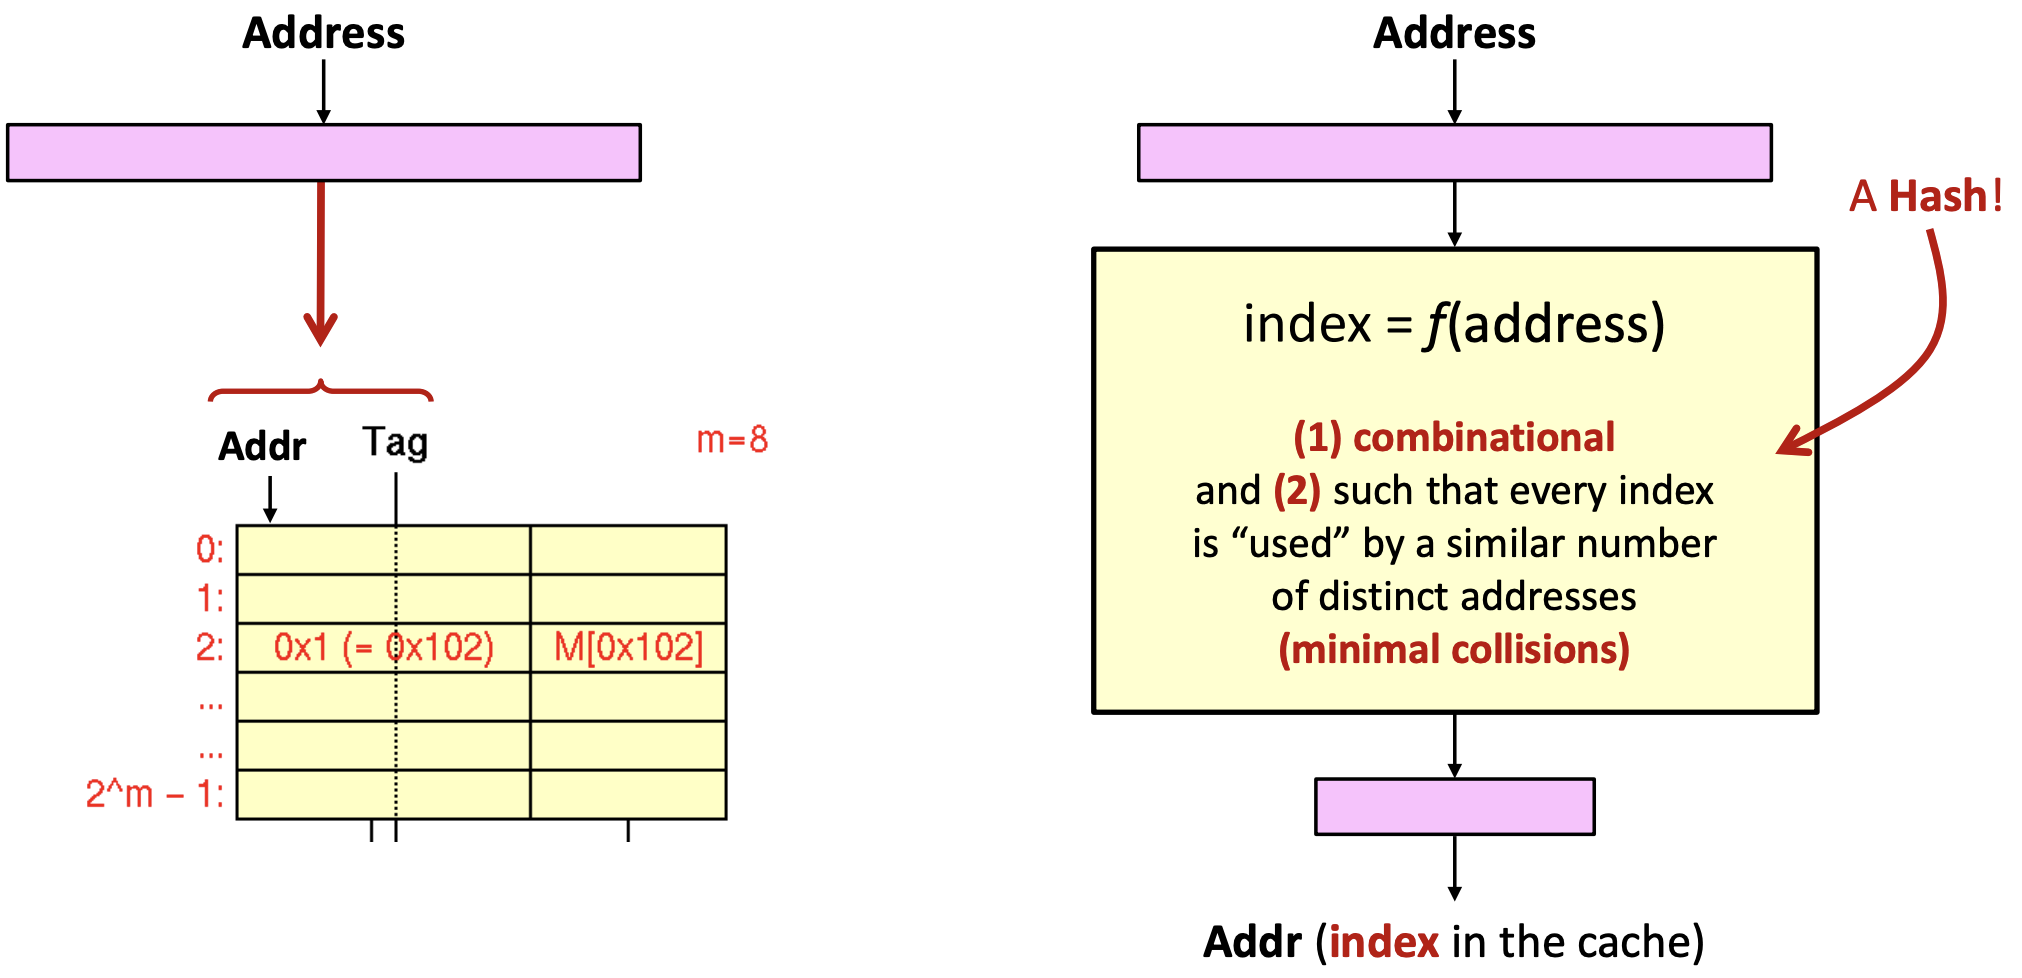
\includegraphics[width=0.65\textwidth]{chapters/chapter3a/images/gen.png}
\end{center}
\begin{itemize}
    \item \textbf{\texttt{Addr} (Index in Cache):}
    \begin{itemize}
        \item The \texttt{Addr} is derived using a function \( f(\texttt{Address}) \), typically a hash function.
        \item Properties of \( f(\texttt{Address}) \):
        \begin{itemize}
            \item It is combinational (fast to compute).
            \item It distributes memory addresses uniformly across cache indices to minimize collisions.
        \end{itemize}
        \item Example: For \texttt{0x102}, the computed \texttt{Addr} is the index in the cache where the block will reside.
    \end{itemize}

    \item \textbf{\texttt{Tag} (Identification of the Block):}
    \begin{itemize}
        \item The \texttt{Tag} represents the higher-order bits of the memory address, used to verify if the desired data resides in the indexed cache line.
        \item For example, the \texttt{Tag} for \texttt{0x102} is \texttt{0x1}.
    \end{itemize}

    \item \textbf{Hashing for \texttt{Addr} Generation:}
    \begin{itemize}
        \item A well-designed hash function ensures:
        \begin{itemize}
            \item Minimal collisions: Every cache index is mapped to by a similar number of distinct addresses.
            \item Efficient access: Avoids excessive contention for cache lines.
        \end{itemize}
    \end{itemize}
\end{itemize}

\subsection{The Simplest Hash Function}
The simplest hashing schemes involve deriving an \textit{Index} from an \textit{Address} of $n$ bits by selecting $m$ bits. Two common approaches for selecting these $m$ bits are as follows:
\begin{center}
    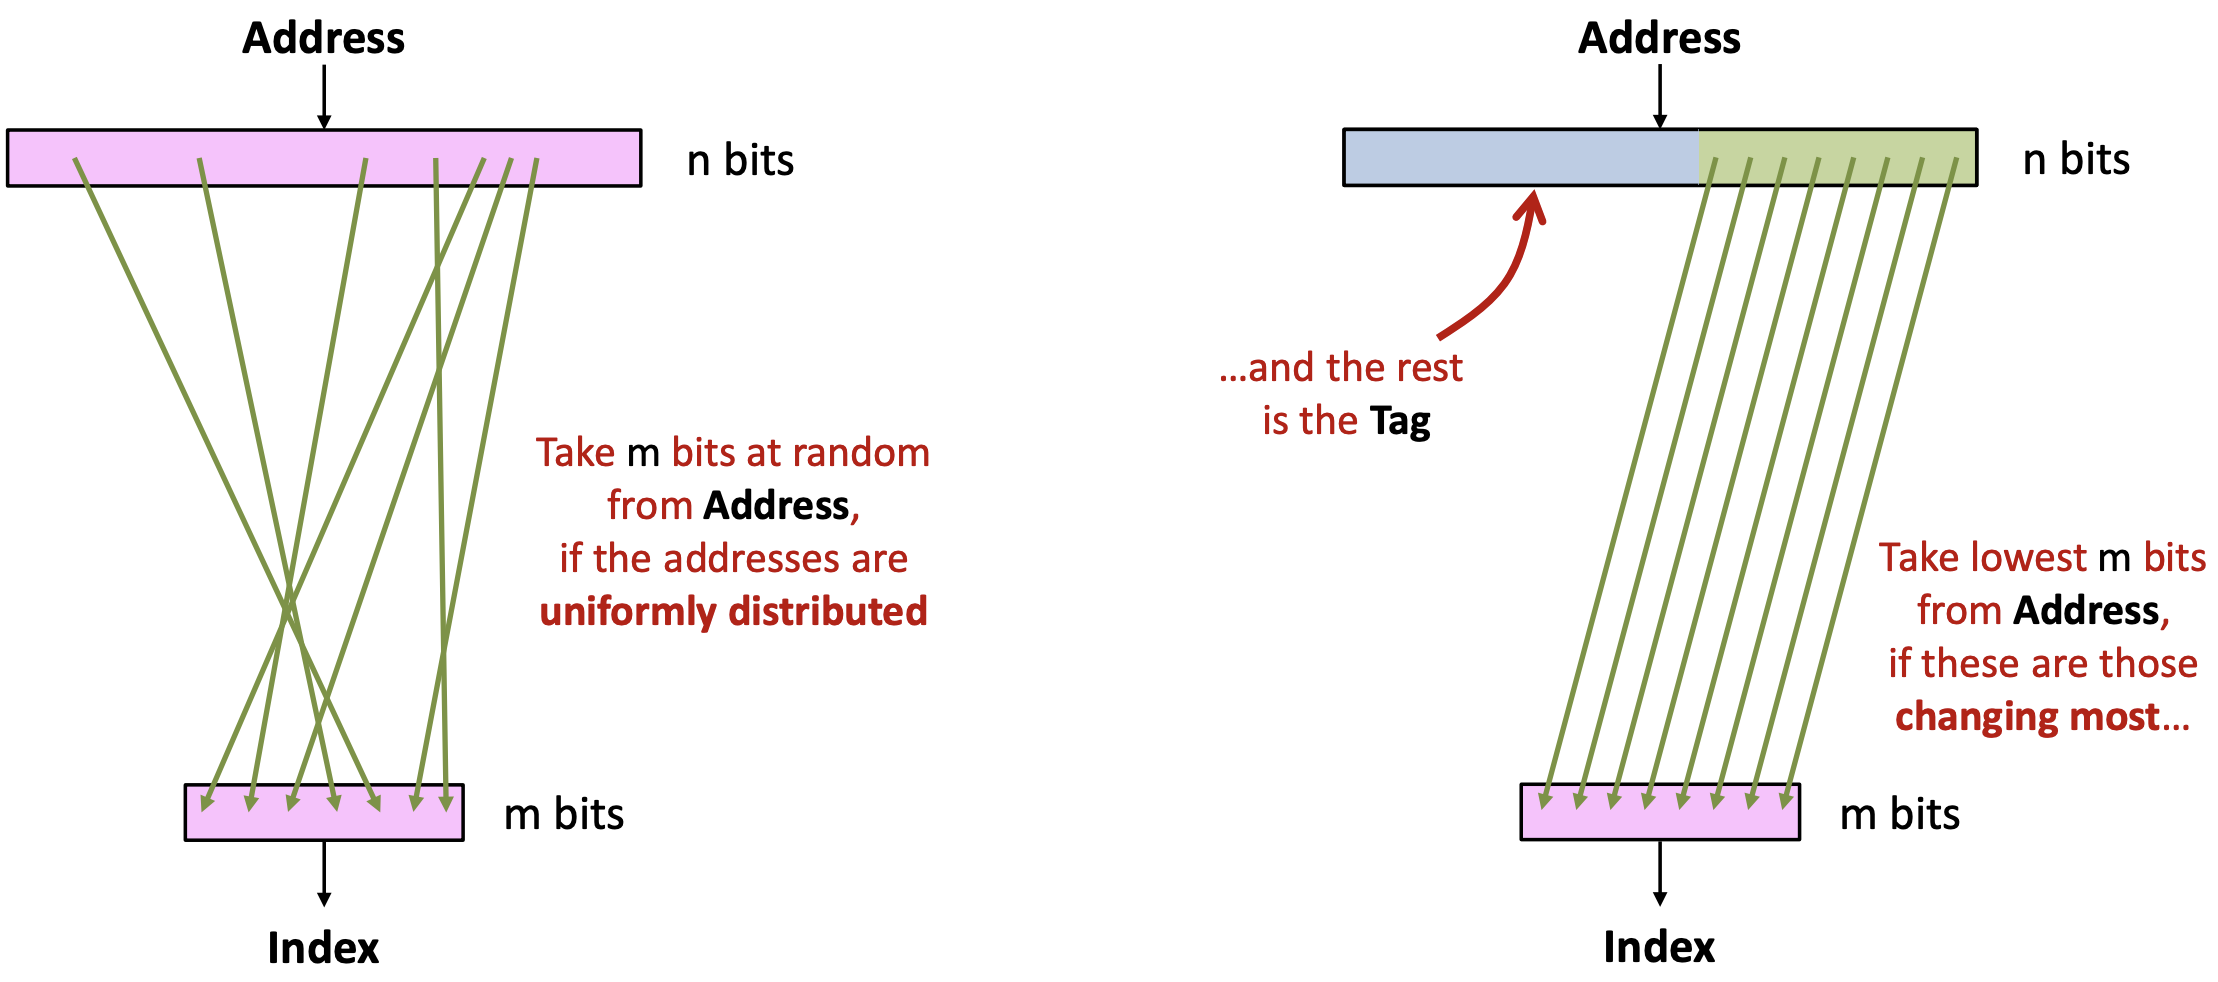
\includegraphics[width=0.45\textwidth]{chapters/chapter3a/images/hash.png}
\end{center}
\begin{itemize}
    \item \textbf{Random Selection:} Choose $m$ bits at random from the $n$-bit \textit{Address}, provided the addresses are uniformly distributed. This random selection ensures an even distribution of indices.
    
    \item \textbf{Lowest Bits Selection:} Select the $m$ least significant bits (LSBs) from the \textit{Address}. This method is particularly effective when the lower bits of the \textit{Address} are those that change the most frequently.
\end{itemize}

Once the $m$ bits are extracted to form the \textit{Index}, the remaining $(n-m)$ bits constitute the \textit{Tag}. The \textit{Tag} can be used for further identification or verification processes.

\subsubsection{Direct-Mapped Cache}
A \textit{Direct-Mapped Cache} is a simplified and cost-effective approach to caching that uses the \textit{Address} to directly index into a specific cache line. This scheme divides the \textit{Address} into two parts:
\begin{center}
    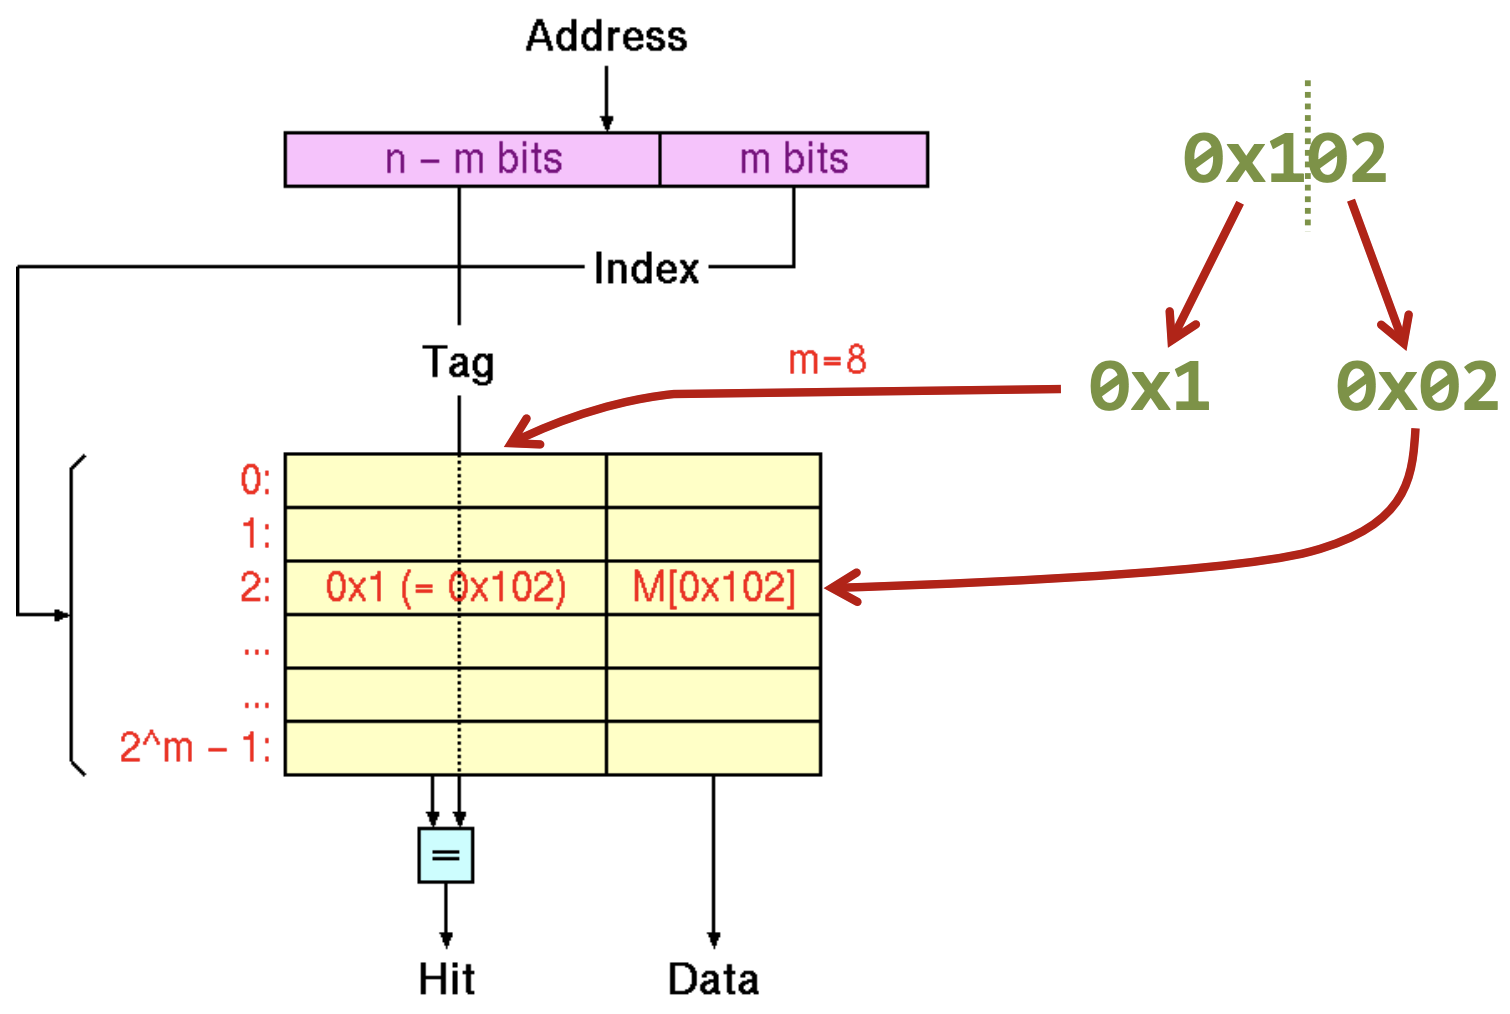
\includegraphics[width=0.45\textwidth]{chapters/chapter3a/images/dmc.png}
\end{center}
\begin{itemize}
    \item \textbf{Index ($m$ bits):} Specifies the cache line where the data is stored.
    \item \textbf{Tag ($n-m$ bits):} Identifies whether the cache line corresponds to the requested memory address.
\end{itemize}

The process of accessing the cache is as follows:
\begin{enumerate}
    \item The \textit{Index} is derived from the $m$ least significant bits of the \textit{Address}.
    \item The corresponding cache line is checked, and the \textit{Tag} is compared to validate the match.
    \item If the \textit{Tag} matches, it is a \textit{cache hit}, and the requested data is fetched.
    \item Otherwise, it is a \textit{cache miss}, and the data must be retrieved from the main memory.
\end{enumerate}
\newpage
\section{Which One is the Best Cache ?}
\textbf{Objective:} Analyze the hit rate of two types of caches: \textit{fully associative} and \textit{direct-mapped}, given the following scenario.
\begin{center}
    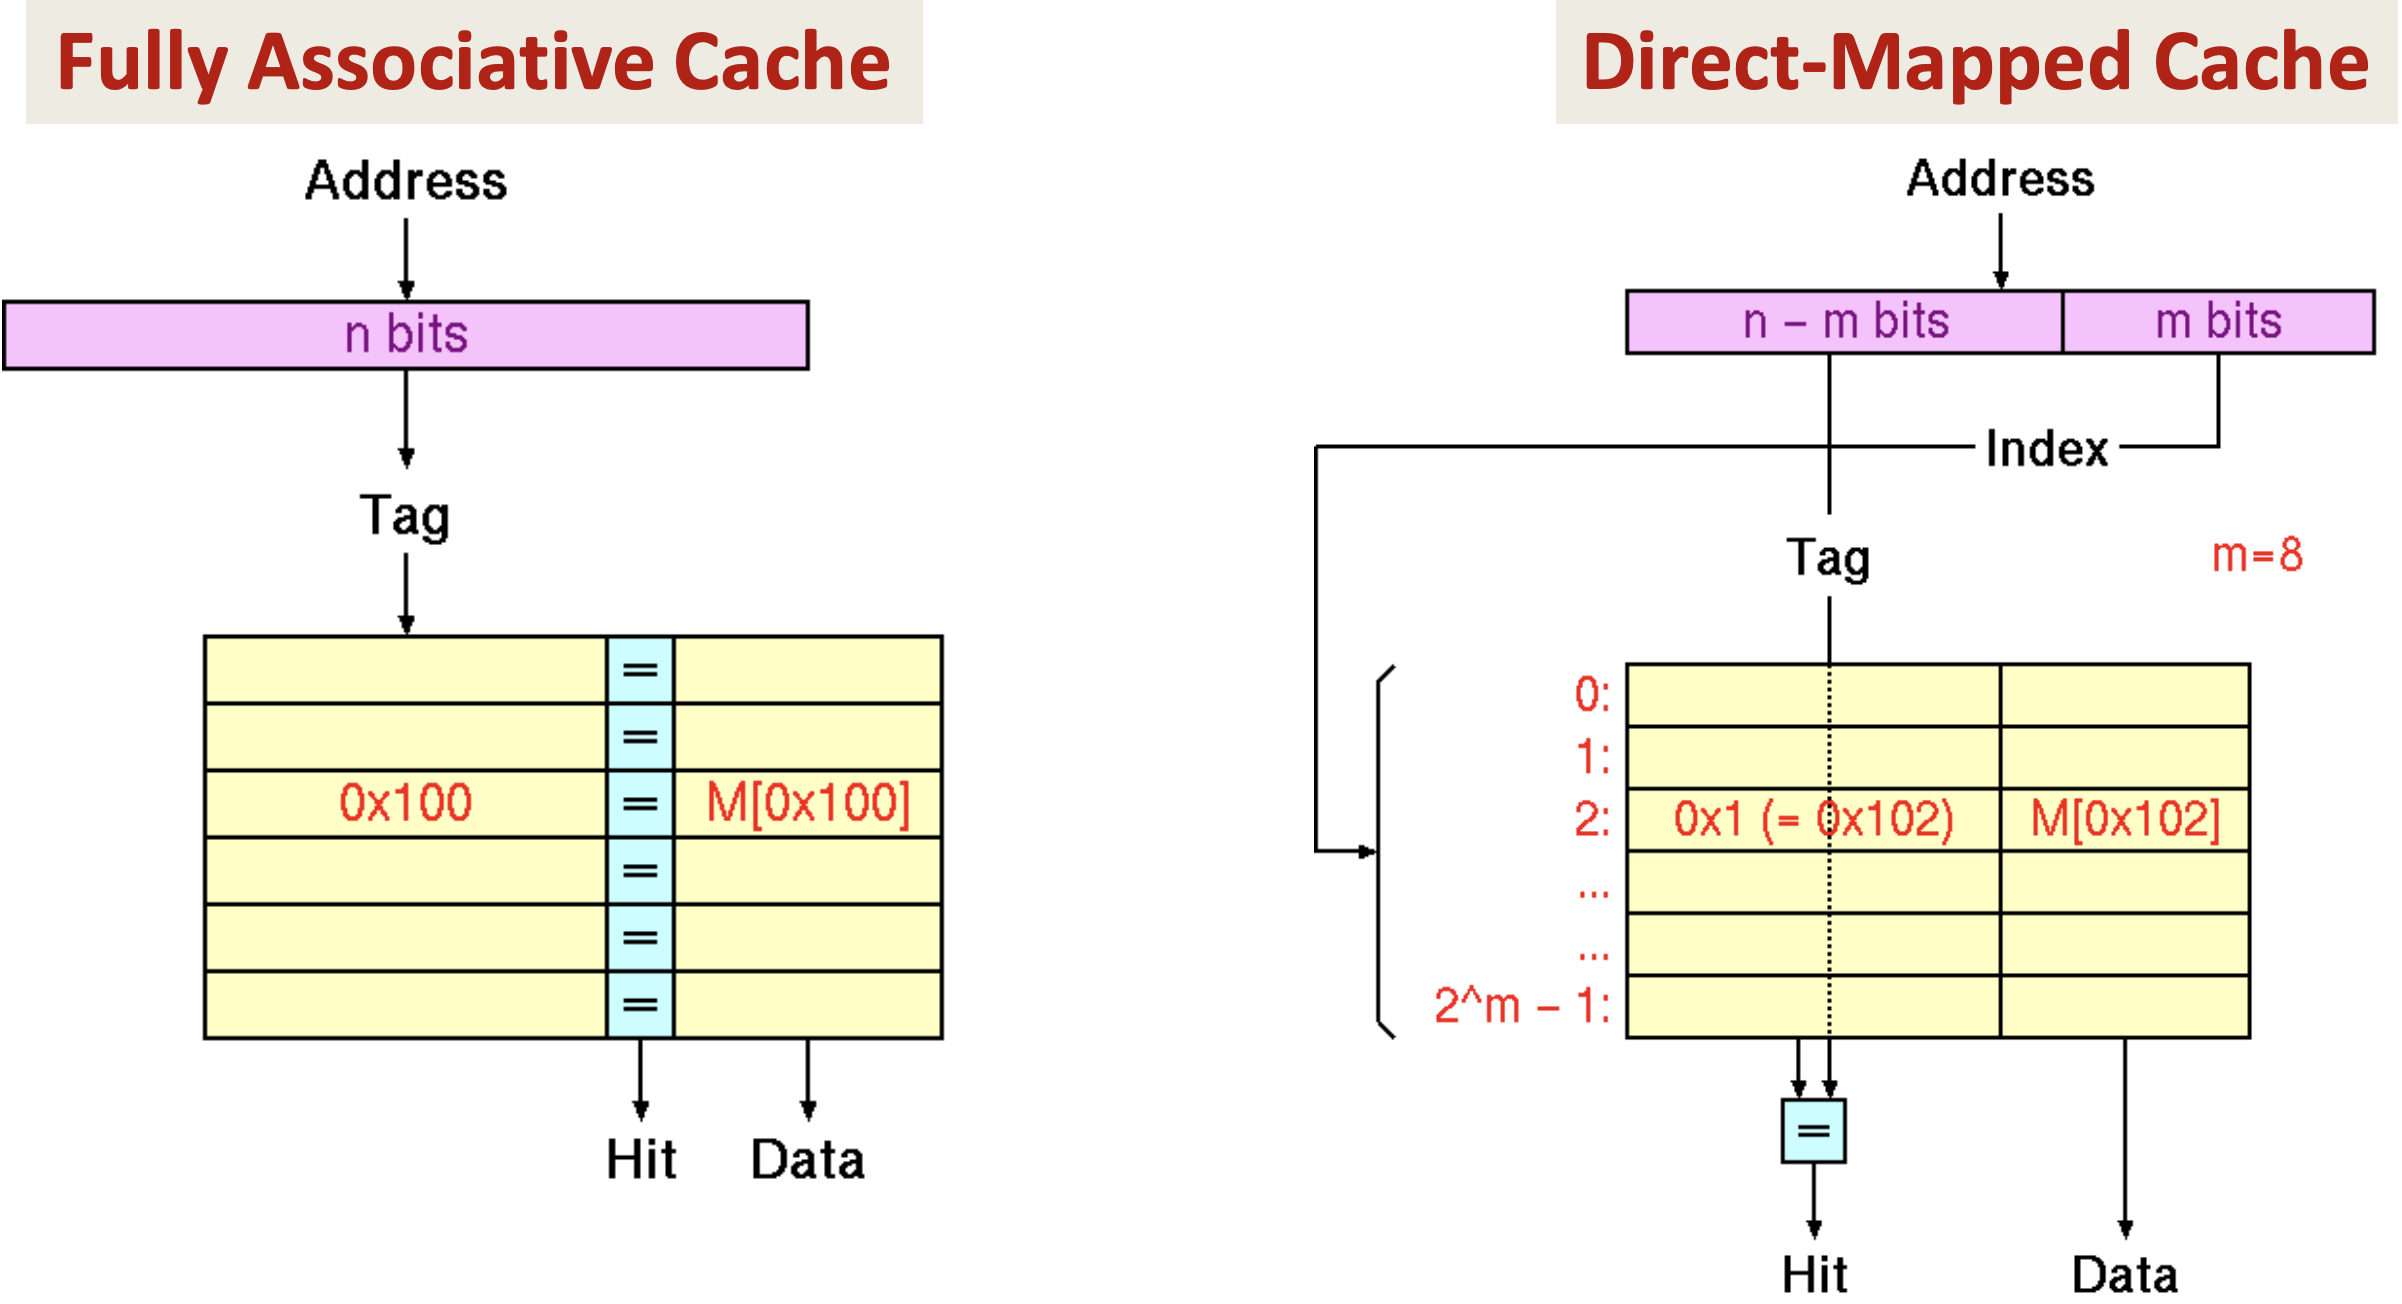
\includegraphics[width=0.65\textwidth]{chapters/chapter3a/images/best.png}
\end{center}
\begin{center}
    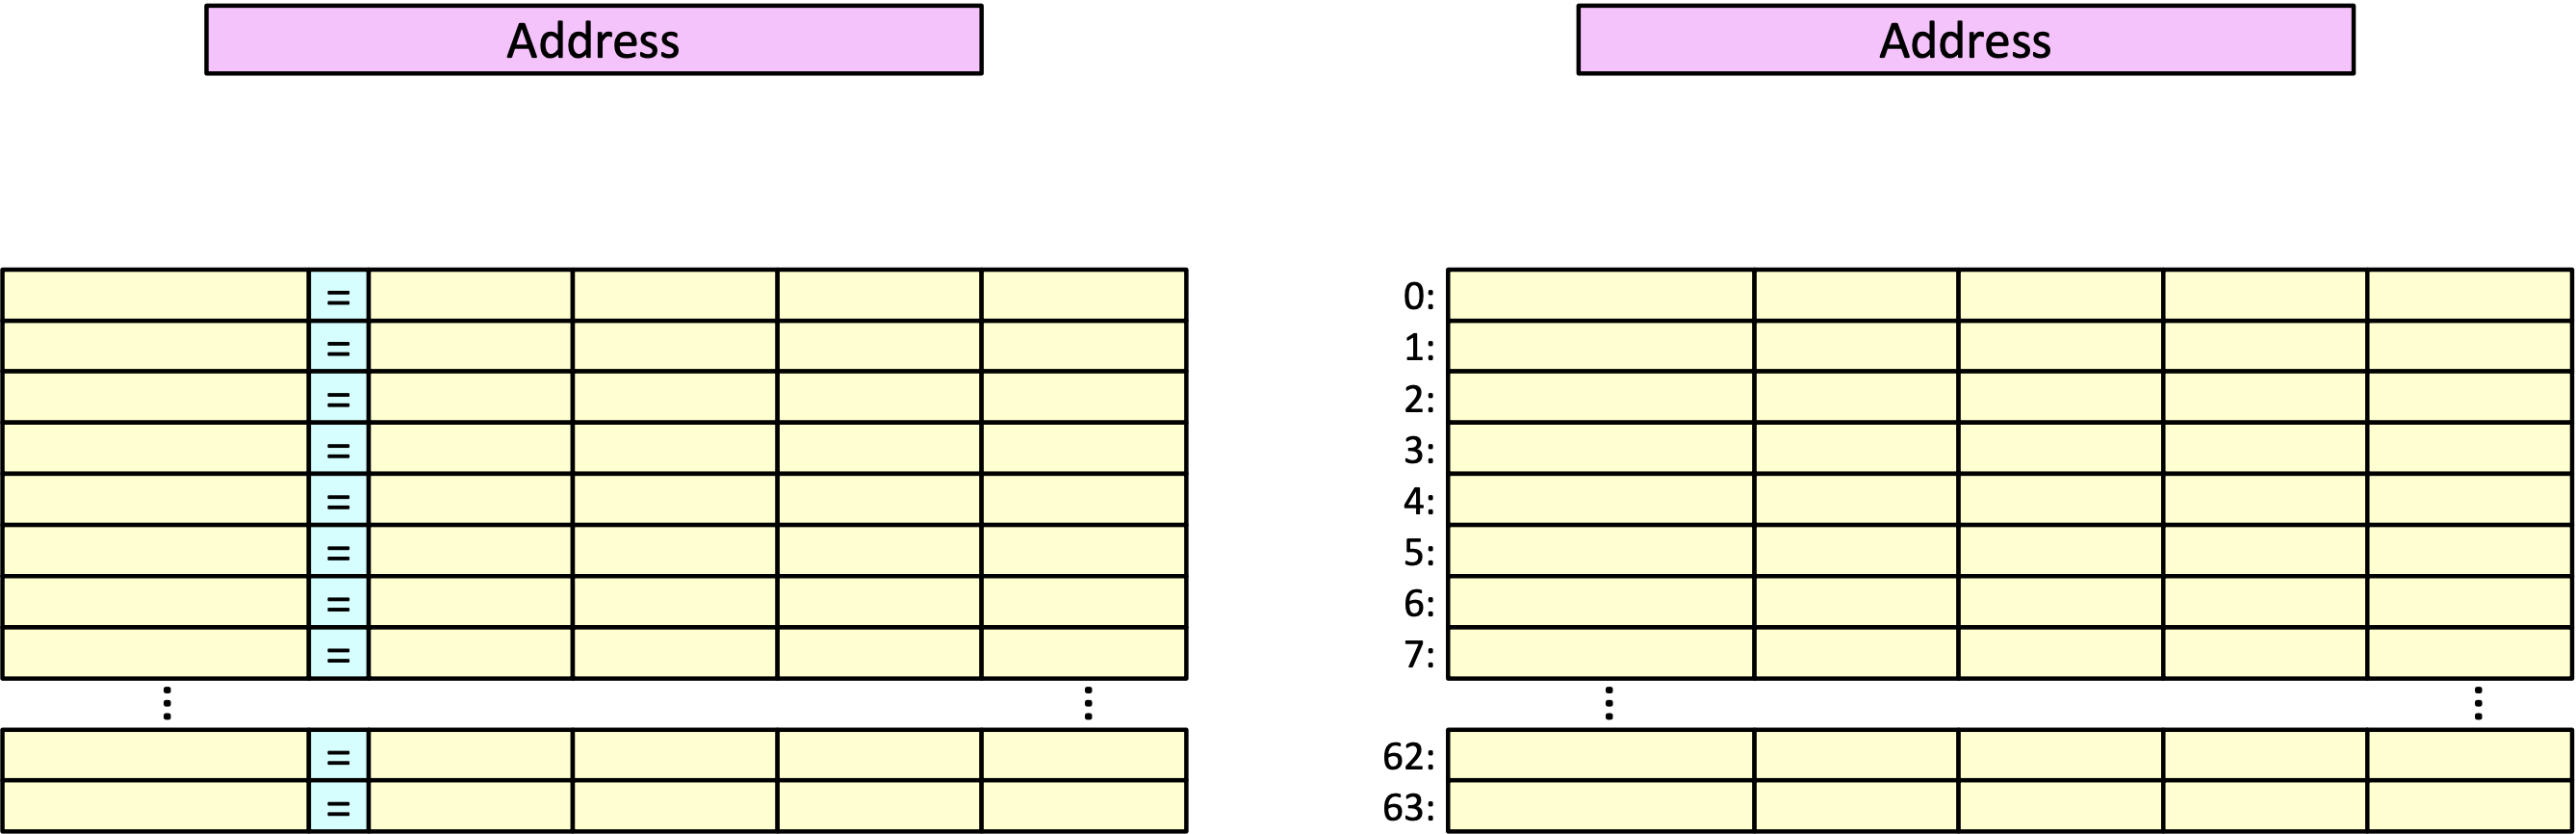
\includegraphics[width=0.65\textwidth]{chapters/chapter3a/images/example.png}
\end{center}
\textbf{Cache Details:}
\begin{itemize}
    \item Both caches have 64 lines with four words per line, resulting in a total of 256 words per cache.
    \item Addresses accessed sequentially: \texttt{0x100}, \texttt{0x101}, \texttt{0x200}, \texttt{0x102}, \texttt{0x300}, \texttt{0x103}, \texttt{0x201}, \texttt{0x102}, \texttt{0x301}, \texttt{0x103}, \dots
\end{itemize}

\textbf{Cache Architectures:}
\begin{enumerate}
    \item \textbf{Fully Associative Cache:} Any block can be stored in any cache line. Blocks are located using a tag comparison.
    \item \textbf{Direct-Mapped Cache:} Each memory block maps to exactly one cache line, determined by the lower $m$ bits of the address (index), where $m = 8$.
\end{enumerate}

\textbf{Analysis:}
\begin{itemize}
    \item \textbf{Fully Associative Cache:} As the cache has no fixed mapping of addresses to lines, it can utilize its capacity efficiently. Cache replacement policies (e.g., LRU) determine which block to evict upon a miss.
    \item \textbf{Direct-Mapped Cache:} Due to fixed mappings, cache conflicts occur when multiple addresses map to the same index. This can result in more frequent misses, even if the cache is not fully utilized.
\end{itemize}
ima
\textbf{Question:} What is the \textbf{hit rate} of each cache under the given access sequence?
\begin{center}
    \begin{tabular}{|c|c|c|c|c|c|c|c|c|c|c|}
    \hline
    \textbf{} & \textbf{0x100} & \textbf{0x101} & \textbf{0x200} & \textbf{0x102} & \textbf{0x300} & \textbf{0x103} & \textbf{0x201} & \textbf{0x102} & \textbf{0x301} & \textbf{0x103} \\ \hline
    \textbf{Fully Ass.} & M & H & M & H & M & H & H & H & H & H \\ \hline
    \textbf{Direct Mapp.} & M & H & M & M & M & M & M & M & M & M \\ \hline
    \end{tabular}
\end{center}
    
\textbf{Calculation of the First Three Memory Accesses:}
\begin{enumerate}
    \item \textbf{Access to \texttt{0x100}:}
    \begin{itemize}
        \item \textbf{Fully Associative Cache:} Since the cache is initially empty, this is a \textbf{miss}. The block containing \texttt{0x100} is loaded into the cache.
        \item \textbf{Direct-Mapped Cache:} The cache line index is calculated using the lower 8 bits of the address (after accounting for block offset). Assuming a block size of 4 words (i.e., 2 bits for block offset), the index is:
        \[
        \text{Index} = \left( \frac{\texttt{0x100}}{4} \right) \mod 64 = 64 \mod 64 = 0
        \]
        This is a \textbf{miss}, and the block is loaded into cache line 0.
    \end{itemize}
    \item \textbf{Access to \texttt{0x101}:}
    \begin{itemize}
        \item \textbf{Fully Associative Cache:} The block containing \texttt{0x100} also contains \texttt{0x101} (since they are in the same block). This is a \textbf{hit}.
        \item \textbf{Direct-Mapped Cache:} \texttt{0x101} maps to the same cache line as \texttt{0x100}. It's within the same block already loaded, resulting in a \textbf{hit}.
    \end{itemize}
    \item \textbf{Access to \texttt{0x200}:}
    \begin{itemize}
        \item \textbf{Fully Associative Cache:} This address is not in the cache, leading to a \textbf{miss}. The block containing \texttt{0x200} is loaded into the cache.
        \item \textbf{Direct-Mapped Cache:} The index is calculated as:
        \[
        \text{Index} = \left( \frac{\texttt{0x200}}{4} \right) \mod 64 = 128 \mod 64 = 0
        \]
        \texttt{0x200} maps to cache line 0, the same as \texttt{0x100}. This causes a \textbf{conflict miss} as it replaces the block containing \texttt{0x100} and \texttt{0x101}.
    \end{itemize}
\end{enumerate}

\textbf{Why the Direct-Mapped Cache Misses After \texttt{0x101}:}

In a direct-mapped cache, each block of memory maps to a single cache line based on its index. Addresses \texttt{0x100}, \texttt{0x200}, \texttt{0x300}, etc., share the same index due to their address patterns:

\begin{itemize}
    \item \texttt{0x100} index: $(256 / 4) \mod 64 = 64 \mod 64 = 0$
    \item \texttt{0x200} index: $(512 / 4) \mod 64 = 128 \mod 64 = 0$
    \item \texttt{0x300} index: $(768 / 4) \mod 64 = 192 \mod 64 = 0$
\end{itemize}

This means they all map to cache line 0. After \texttt{0x101}, every new access (\texttt{0x200}, \texttt{0x300}, etc.) conflicts with previous ones, causing the cache line to be continually overwritten. As a result, subsequent accesses that might benefit from cache hits suffer misses instead.

In contrast, the fully associative cache doesn't have fixed mappings. It can store blocks anywhere, avoiding these conflicts and maintaining higher hit rates after the initial misses.

\section{Associativity}
The associativity of a cache defines the number of possible locations in the cache where a single piece of data can be stored. It significantly influences the probability of \textbf{aliasing} (multiple memory addressing maps to the same cache data, causing potential coherency issues or conflicts) in cache memory. For now we've seen :

\begin{itemize}
    \item \textbf{Fully Associative:} Each word can be stored in any line of the cache. This implies that the associativity equals the total number of lines in the cache.
    \item \textbf{Direct Mapped:} Each word is mapped to exactly one line in the cache. Thus, the associativity in this case is 1.
\end{itemize}
but maybe there is a better one\dots

\newpage
\subsection{Set-Associative Cache}
A \textbf{set-associative cache} combines features of both direct-mapped and fully associative caches. It divides the cache into multiple sets, where each set contains a fixed number of blocks known as \textit{ways}. A typical configuration is a \textit{k-way set-associative cache}, where each set can hold up to $k$ blocks.

\begin{center}
    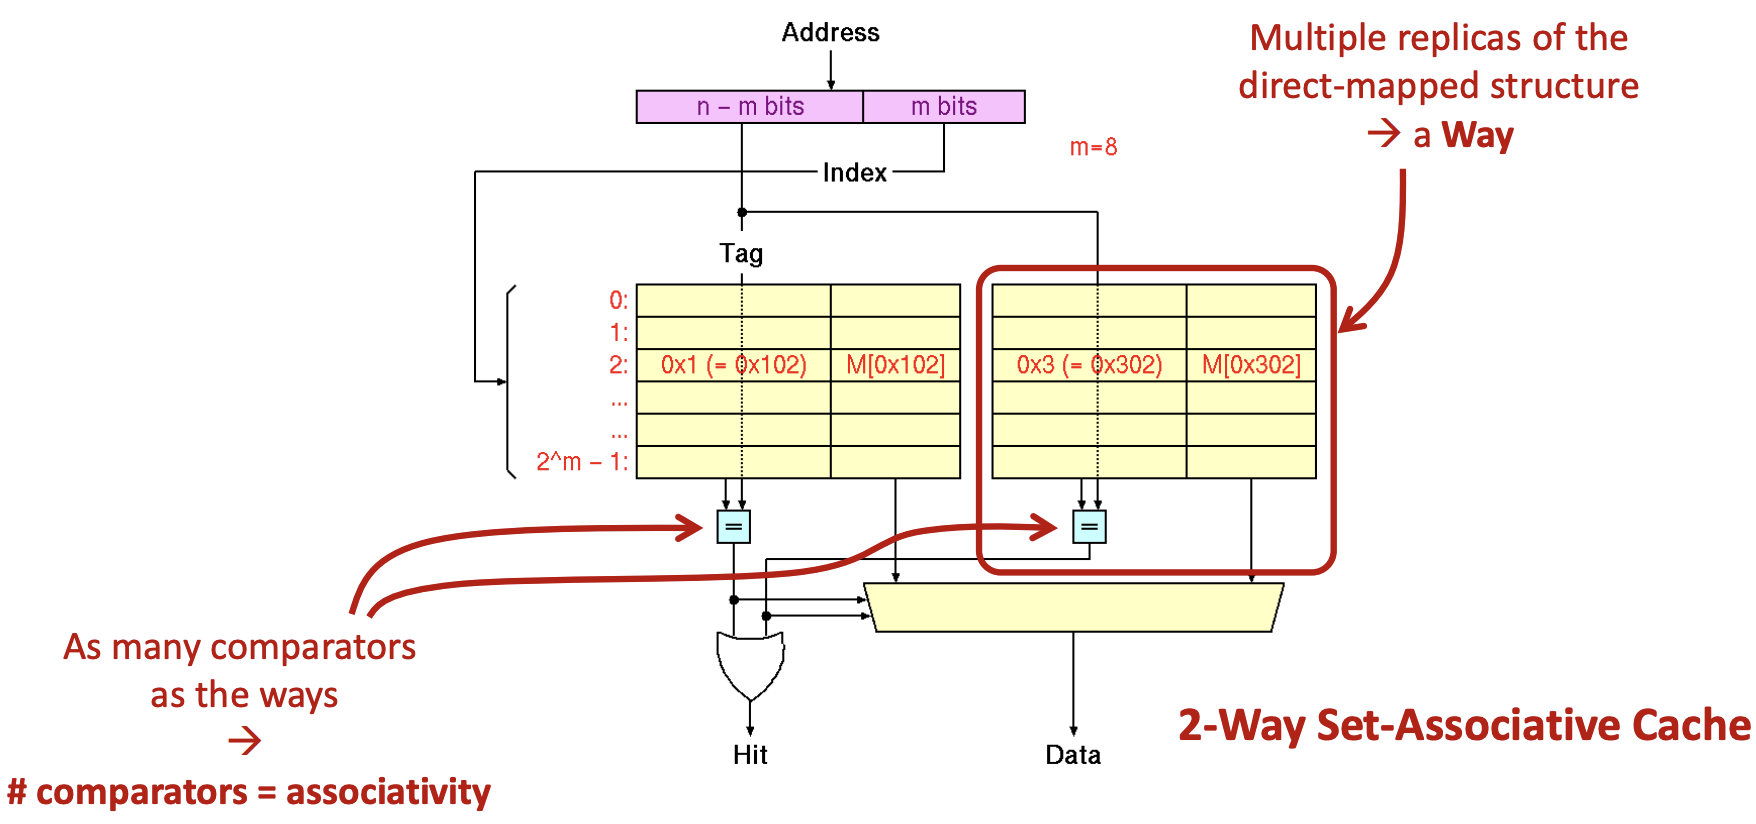
\includegraphics[width=0.65\textwidth]{chapters/chapter3a/images/set.png}
\end{center}

\subsubsection*{Address Breakdown}
The memory address is divided into three fields:
\begin{itemize}
    \item \textbf{Tag:} Identifies whether a particular block is in the cache.
    \item \textbf{Index:} Specifies the set to which the block belongs.
    \item \textbf{Offset:} Specifies the location within a block.
\end{itemize}

\subsubsection*{Structure and Operation}
Each set operates as a miniature associative cache, allowing multiple blocks to reside in the same set. The operation involves:
\begin{itemize}
    \item \textbf{Comparison:} A comparator is used for each way to check if the tag of a block in the cache matches the tag from the memory address.
    \item \textbf{Hit Detection:} If any comparator signals a match, a \textit{cache hit} occurs, and the corresponding data is retrieved.
    \item \textbf{Miss Handling:} If no match is found, a \textit{cache miss} occurs, and the block is fetched from the next level of memory and stored in the appropriate set.
\end{itemize}

\subsubsection*{2-Way Set-Associative Cache}
A common configuration is the \textbf{2-way set-associative cache}, where each set contains two blocks. This design reduces conflicts compared to direct-mapped caches while maintaining lower complexity than fully associative caches.

\textbf{Key Features:}
\begin{itemize}
    \item Multiple replicas of the direct-mapped structure form the \textit{ways}.
    \item The number of comparators equals the number of ways (\#Comparators = Associativity).
    \item Flexible block placement within a set reduces conflict misses.
\end{itemize}

\subsubsection*{Example: Index Taken in One Way and Not in Another}
In a \textit{2-way set-associative cache}, the following scenario can occur:
\begin{itemize}
    \item \textbf{First Way:} The index points to a block, but the tag stored in the block does not match the tag from the memory address. In this case, the block in the first way is ignored.
    \item \textbf{Second Way:} The index points to an empty block (i.e., the block is not taken). Since there is no valid data in this block, no tag comparison is performed.
\end{itemize}

When neither way results in a tag match or valid data, a \textit{cache miss} occurs. The requested block is then fetched from the next memory level and stored in the appropriate set. Typically, a \textit{replacement policy} (e.g., Least Recently Used, LRU) determines which block in the set will be evicted if the set is full.

\subsection{A Continuum of Possibilities}
\begin{center}
    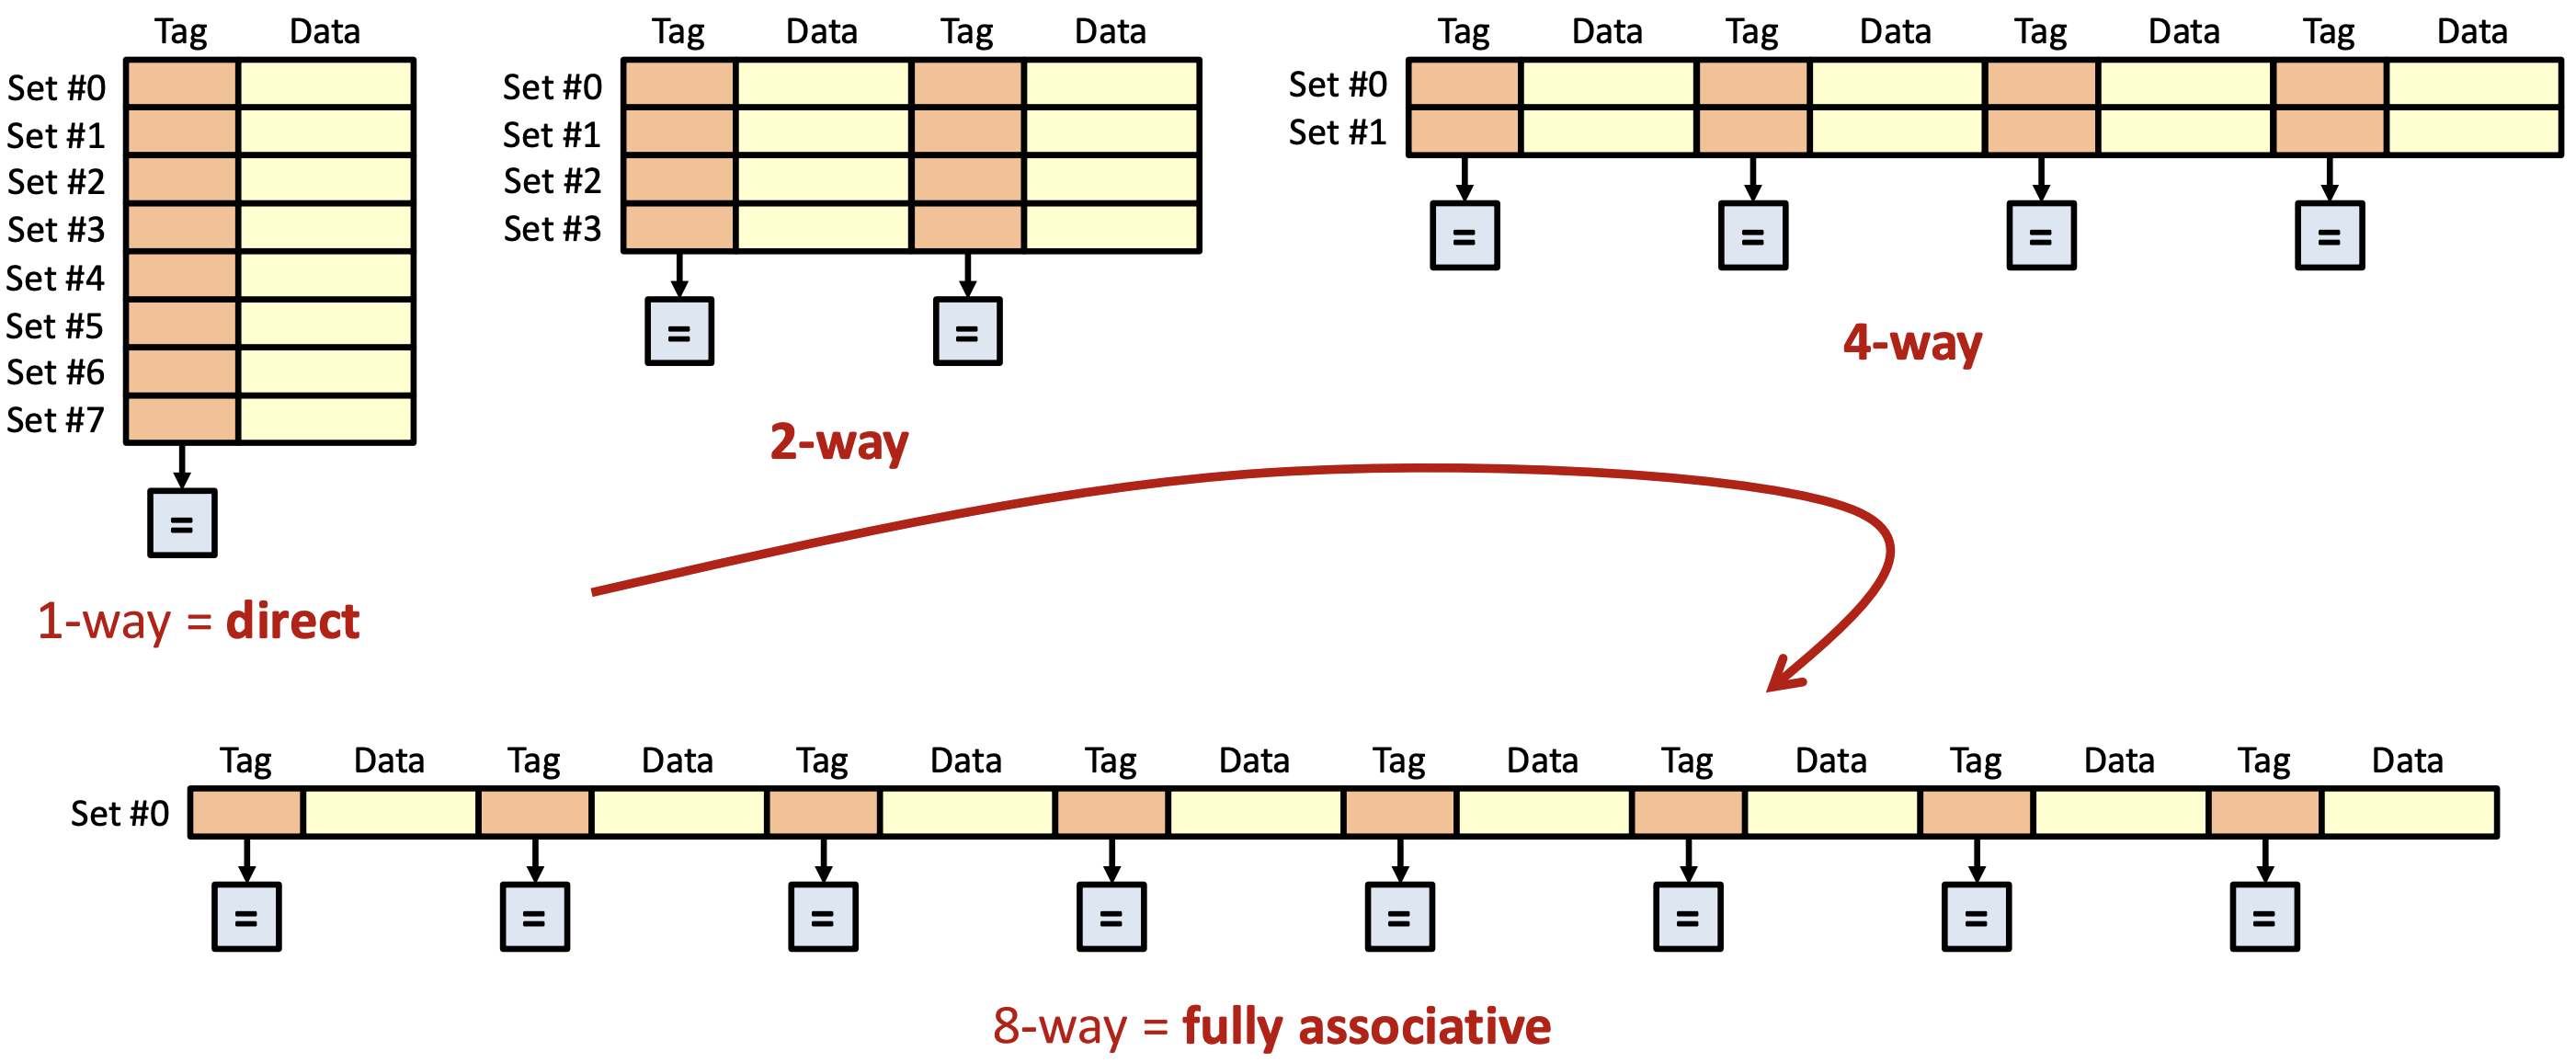
\includegraphics[width=0.65\textwidth]{chapters/chapter3a/images/posib.png}
\end{center}

\begin{itemize}
    \item \textbf{Direct-Mapped Cache (1-way):} Each memory block is mapped to exactly one cache line. This simple design ensures fast access but suffers from higher conflict misses.
    \item \textbf{Set-Associative Cache (N-way):} Memory blocks are mapped to a set of cache lines. Each set can hold \( N \) blocks, reducing conflict misses while introducing moderate hardware complexity. Common examples include:
    \begin{itemize}
        \item \textit{2-way set associative:} Each set contains 2 cache lines.
        \item \textit{4-way set associative:} Each set contains 4 cache lines.
    \end{itemize}
    \item \textbf{Fully Associative Cache (8-way):} Any memory block can be placed in any cache line. This maximizes flexibility and minimizes conflict misses but requires costly associative hardware for lookup.
\end{itemize}

The choice of associativity directly impacts the cache's performance and design trade-offs. A fully associative cache offers the lowest miss rate at the expense of higher power and latency, while a direct-mapped cache provides faster access but is prone to frequent conflicts.

\subsection{Cache Validity}

\textbf{Initial State of Cache:} When a cache is initialized, its content is considered garbage. To ensure proper operation, each cache line includes a \textit{Valid Bit}. This special bit indicates whether the data in a specific cache line is meaningful or not.
\begin{center}
    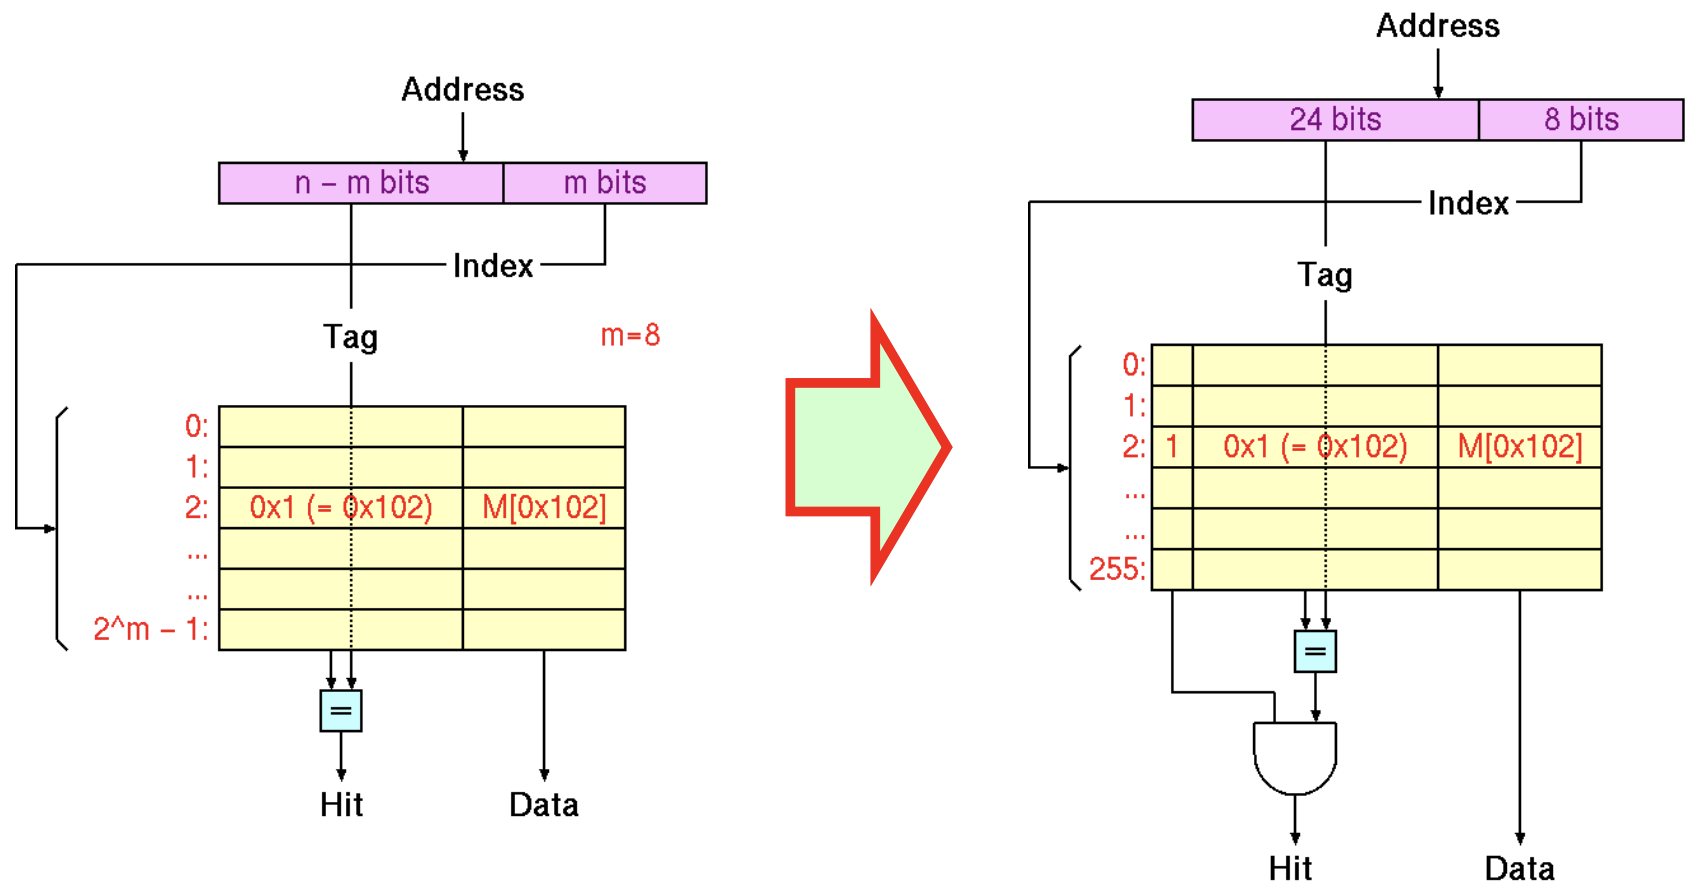
\includegraphics[width=0.65\textwidth]{chapters/chapter3a/images/valid.png}
\end{center}
\textbf{Valid Bit Mechanism:}
\begin{itemize}
    \item The \textit{Valid Bit} is set to \texttt{0} at reset, indicating that the cache line is invalid.
    \item When valid data is written into the cache, the \textit{Valid Bit} is updated to \texttt{1}.
\end{itemize}

\textbf{Cache Hit Check:} To determine if a memory address is present in the cache:
\begin{enumerate}
    \item Compare the \textit{Tag} from the memory address with the \textit{Tag} stored in the indexed cache line.
    \item Ensure the \textit{Valid Bit} of the cache line is set to \texttt{1}.
    \item If both conditions are met, a \textit{Cache Hit} occurs, and the corresponding data is retrieved.
\end{enumerate}

\subsection{Addressing by Byte vs Addressing by Word}
When addressing is \textbf{by byte} and the word size is $2^n$ bytes, the $n$ least-significant bits of the address represent the byte offset. These bits are considered \textbf{irrelevant} for accessing the memory system as they are internal to the processor.
\begin{center}
    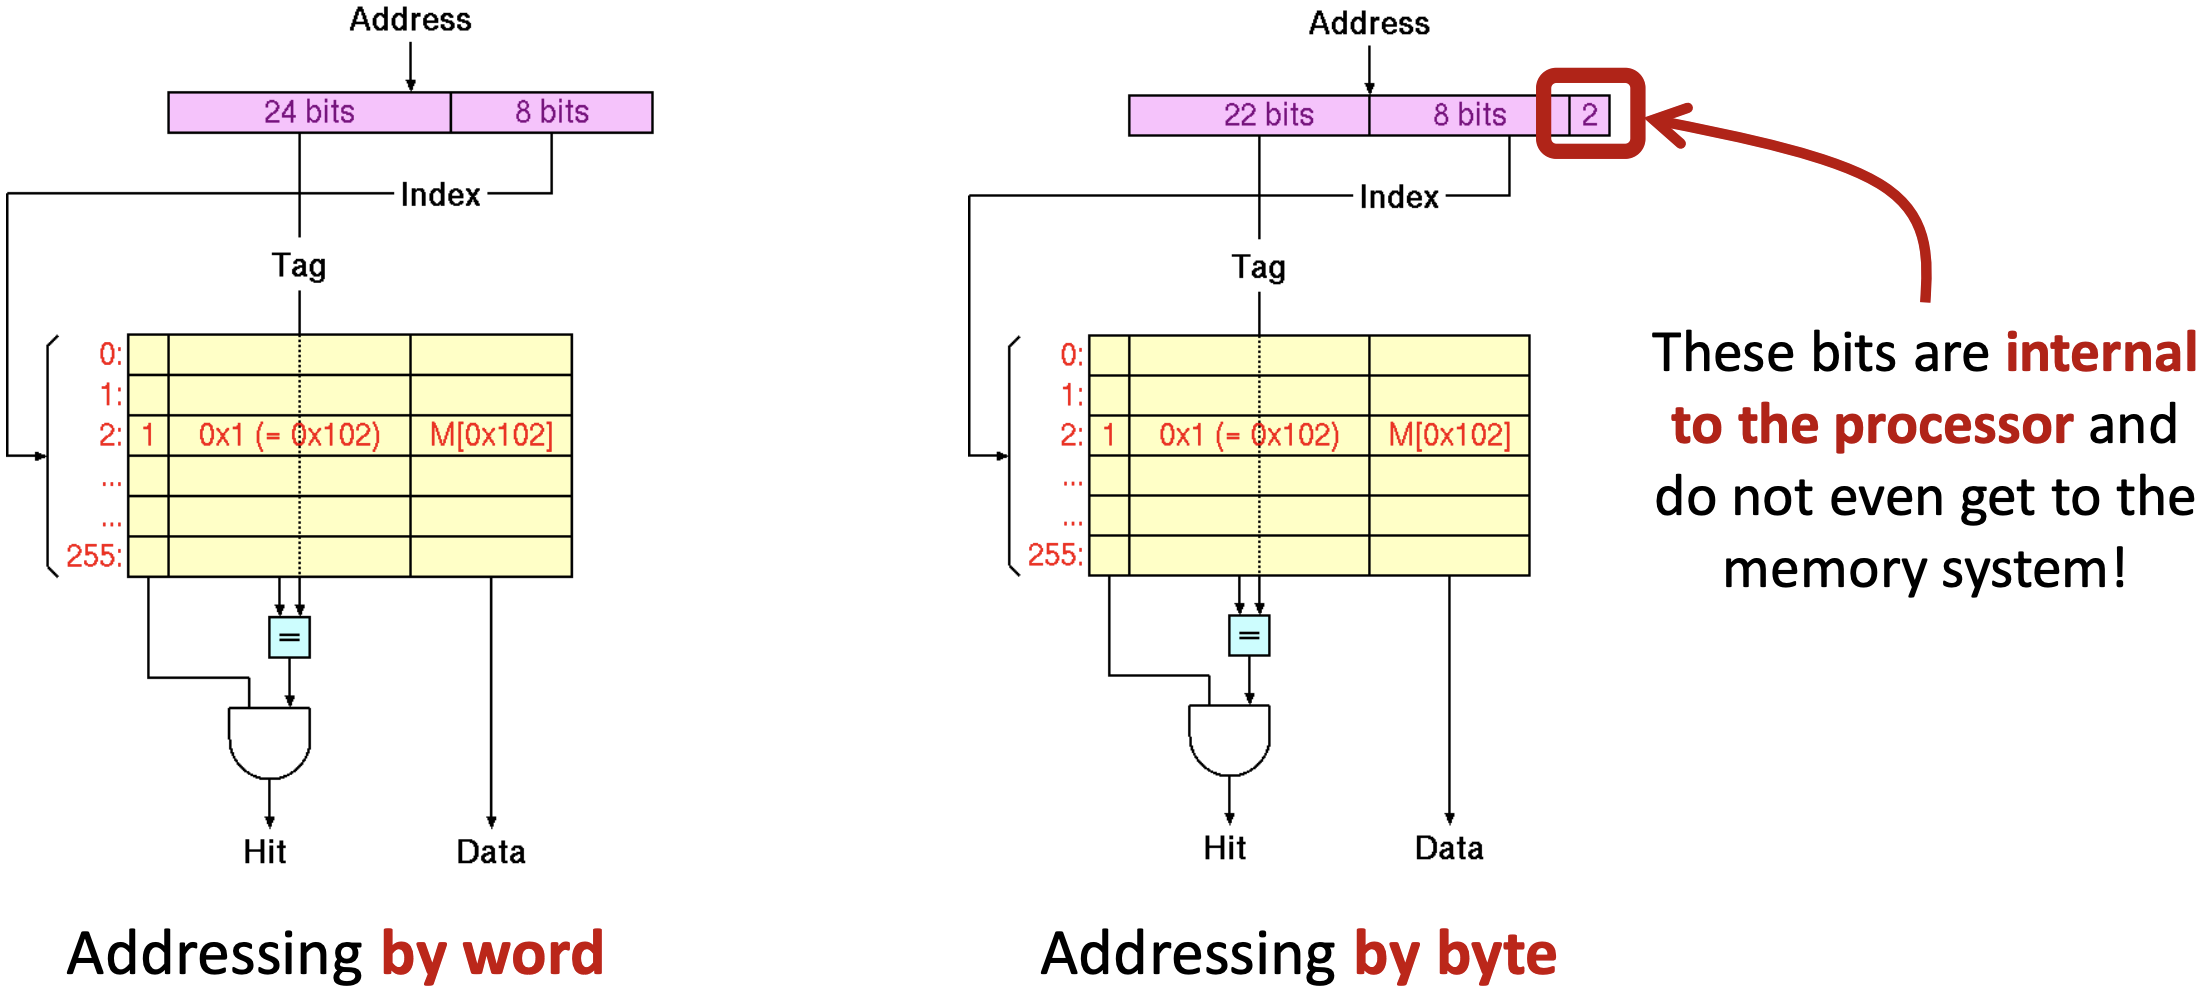
\includegraphics[width=0.65\textwidth]{chapters/chapter3a/images/byte.png}
\end{center}
\begin{itemize}
    \item In \textbf{byte addressing}, the full address includes these $n$ bits, but they do not participate in determining the memory location at the cache level. For example, in the diagram, the 8 least-significant bits are used to compute the offset within a word.
    \item In \textbf{word addressing}, the memory system processes only the address bits beyond the $n$ least-significant bits. The internal processor uses the irrelevant bits for internal data handling but they are not sent to the memory system.
\end{itemize}

\textbf{Key Differences:}
\begin{enumerate}
    \item \textit{Byte Addressing:} All address bits are used to identify individual bytes, ensuring fine-grained access.
    \item \textit{Word Addressing:} The address bits are divided, with the least-significant bits used only internally, simplifying memory system access.
\end{enumerate}

This distinction between addressing schemes impacts cache design and performance, particularly in systems with varying word sizes.

\section{Loading Bytes(lb)}
To load a specific byte from memory into a register, the architecture employs a combination of memory addressing and multiplexing. The process involves the following components:

\begin{center}
    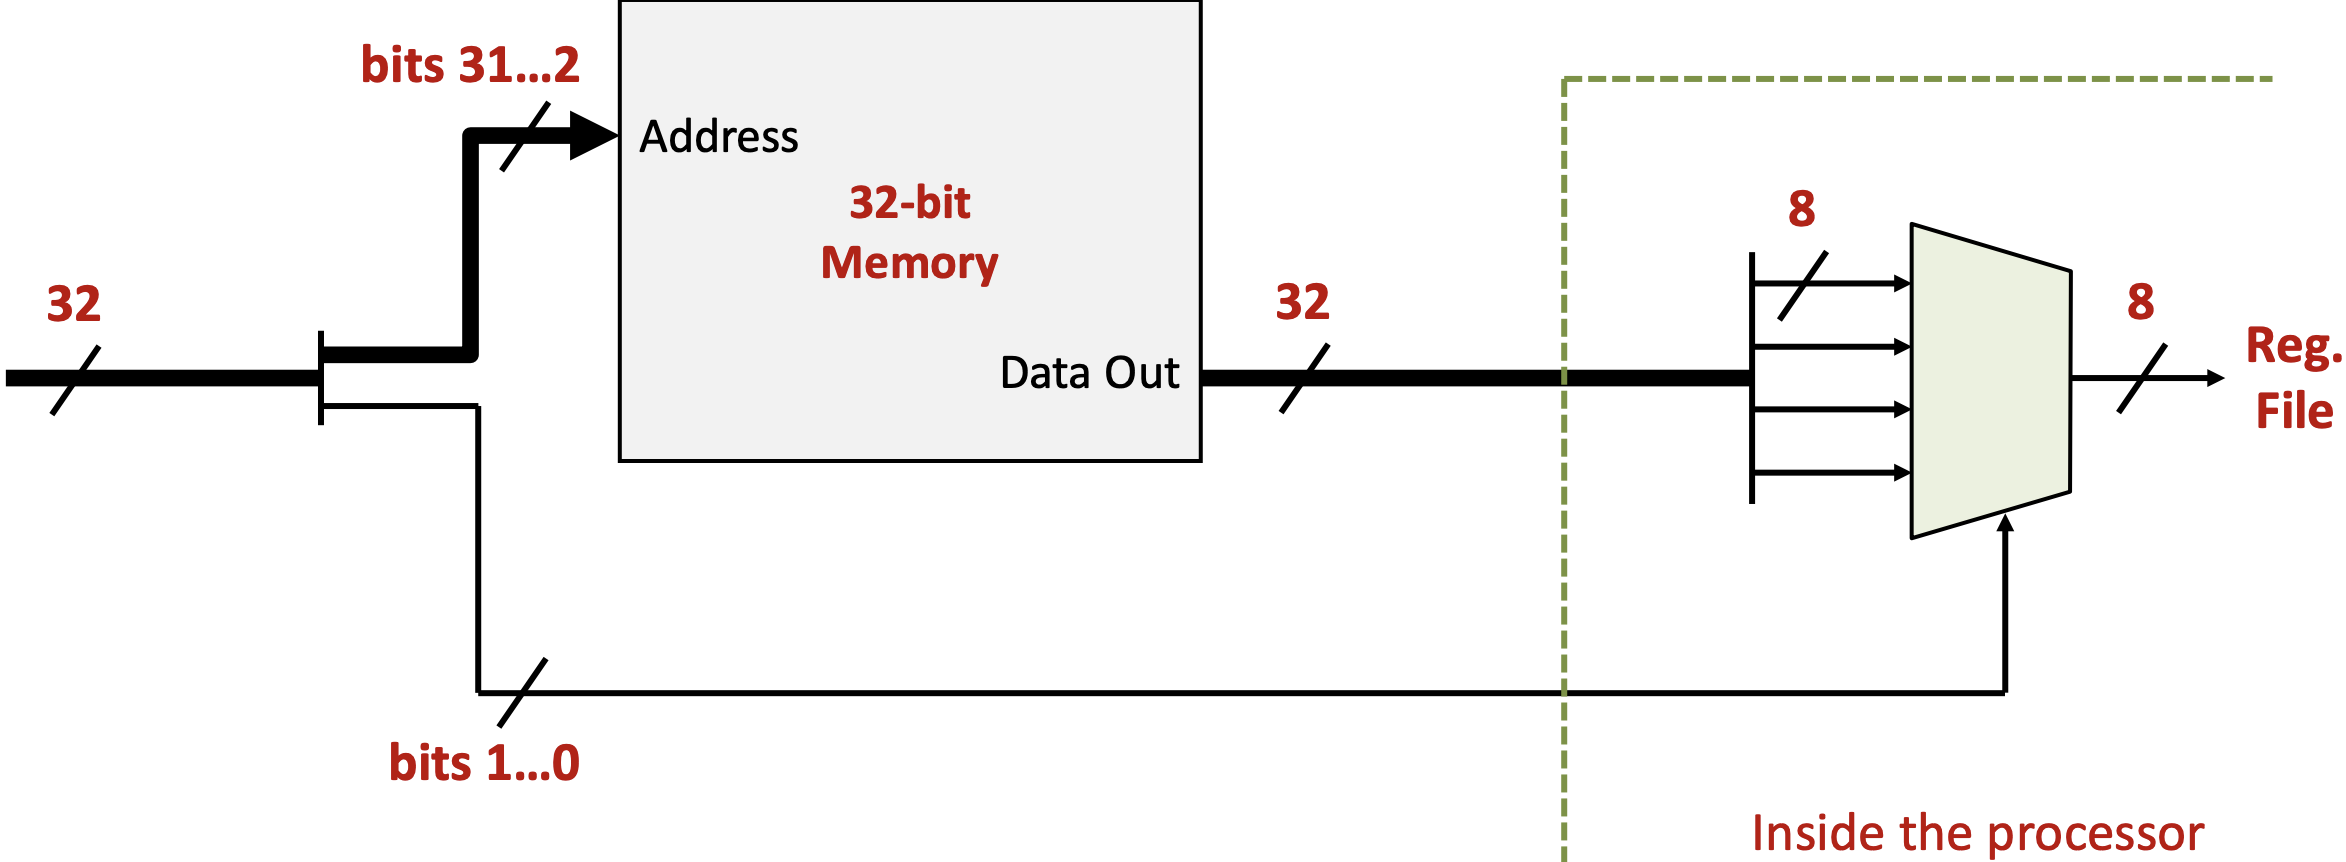
\includegraphics[width=0.65\textwidth]{chapters/chapter3a/images/lb.png}
\end{center}

\begin{itemize}
    \item \textbf{Address Calculation:} The 32-bit memory address is split into two parts:
    \begin{itemize}
        \item \texttt{bits 31...2} specify the base address of the 32-bit memory word.
        \item \texttt{bits 1...0} identify the specific byte within the word.
    \end{itemize}
    \item \textbf{Memory Access:} The calculated address accesses a 32-bit word from memory. The word is then output as \texttt{Data Out}, a 32-bit value.

    \item \textbf{Byte Selection:} A multiplexer extracts the required 8-bit byte from the 32-bit word based on the value of \texttt{bits 1...0}. The multiplexer outputs the selected byte to the processor's register file.

    \item \textbf{Register File Update:} The selected byte is written to the appropriate register within the processor.
\end{itemize}

\subsection{Write Hit}
A \textbf{write hit} occurs when the data to be written is found in the cache. The process involves the following key components and considerations:
\begin{center}
    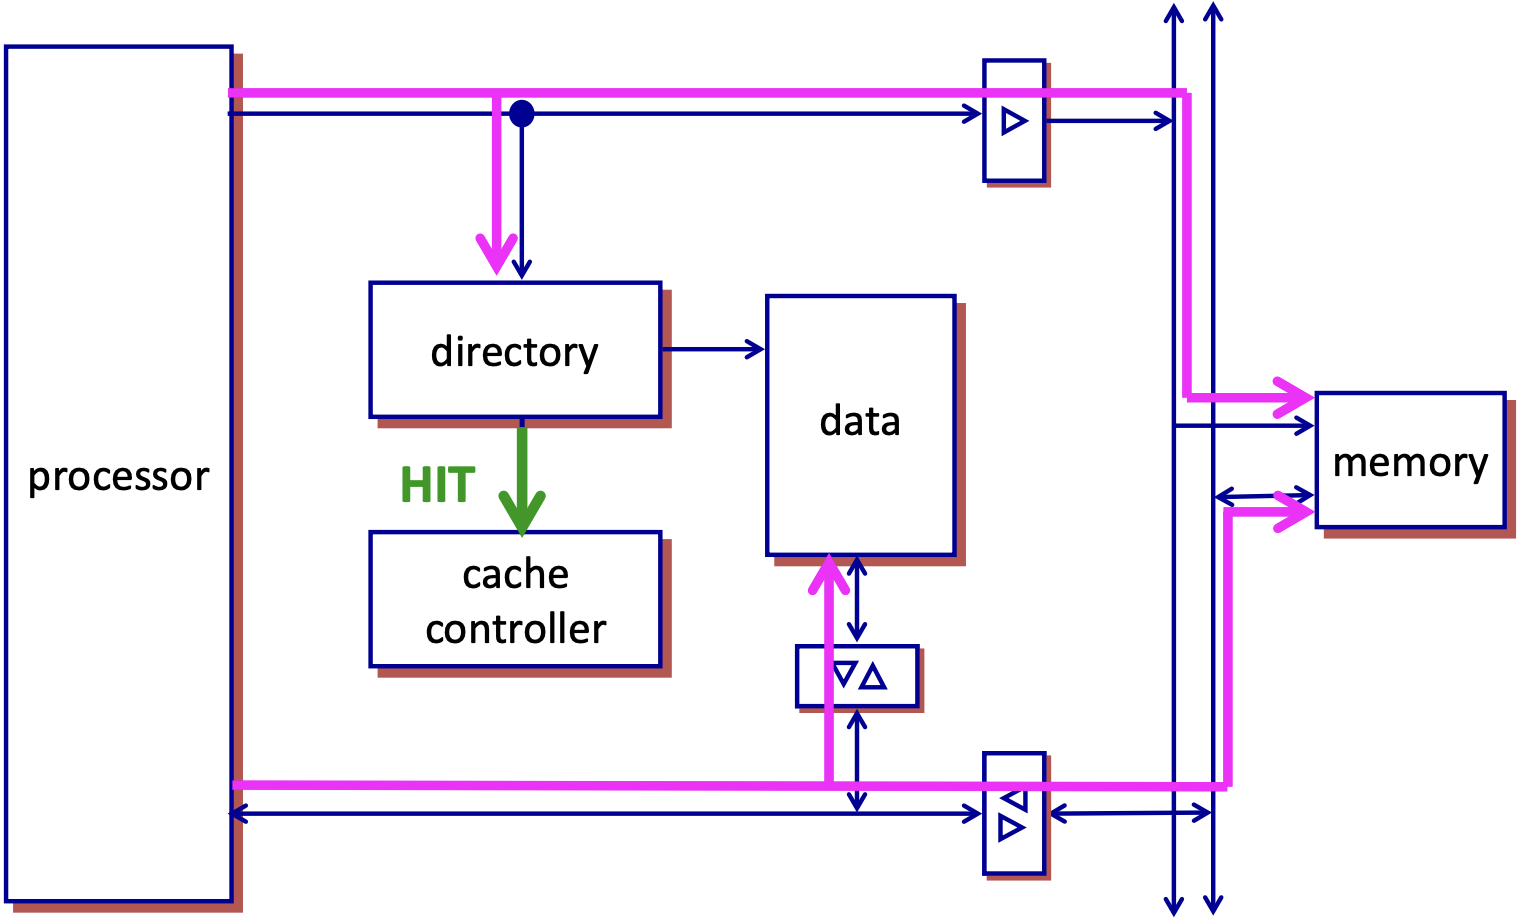
\includegraphics[width=0.45\textwidth]{chapters/chapter3a/images/write_hit.png}
\end{center}

\begin{itemize}
    \item[-] \textbf{Processor Request:} The processor initiates a write operation to a specific address.
    \item[-] \textbf{Cache Lookup:} The \textit{directory} checks if the requested address is present in the cache. Upon finding a match, a \textbf{hit} signal is sent to the \textit{cache controller}.
    \item[-] \textbf{Data Update:} The cache controller updates the data in the cache. The operation ensures that the cache remains consistent with the intended value.
\end{itemize}

An important decision at this stage is whether the data should also be written to the \textit{main memory}. This introduces two potential strategies:
\begin{enumerate}
    \item \textbf{Write-Through:} The updated data is immediately written to both the cache and the main memory, ensuring consistency.
    \item \textbf{Write-Back:} The data is written only to the cache, with changes propagated to the main memory later when the cache block is evicted.
\end{enumerate}
This decision significantly impacts performance and consistency, balancing speed with data reliability. The choice between \textbf{write-through} and \textbf{write-back} is typically determined by the system's design requirements.

\subsubsection{Write Policies in Cache Memory}
When a write operation is performed, the system must decide how to handle the update in the cache and main memory. Two primary write policies are used:

\begin{itemize}
    \item[-] \textbf{Write-Through:}
    \begin{itemize}
        \item Data is immediately written to both the cache and the main memory.
        \item \textbf{Advantages:} Simplifies data consistency between cache and memory.
        \item \textbf{Disadvantages:} Can lead to increased memory traffic, keeping the memory and buses busy unnecessarily.
    \end{itemize}

    \item[-] \textbf{Write-Back (or Copy-Back):}
    \begin{itemize}
        \item Data is only updated in the cache. The main memory remains unchanged until the cache block is evicted.
        \item Requires a \textbf{Dirty Bit} to indicate whether the cached data has been modified.
        \item When a dirty cache line is evicted, it must first be written back to the main memory.
        \item \textbf{Advantages:} Reduces memory write operations, improving performance.
        \item \textbf{Disadvantages:} The main memory may become temporarily inconsistent with the cache.
    \end{itemize}
\end{itemize}

\newpage

\subsection{Write Miss in Cache Memory}
\begin{center}
    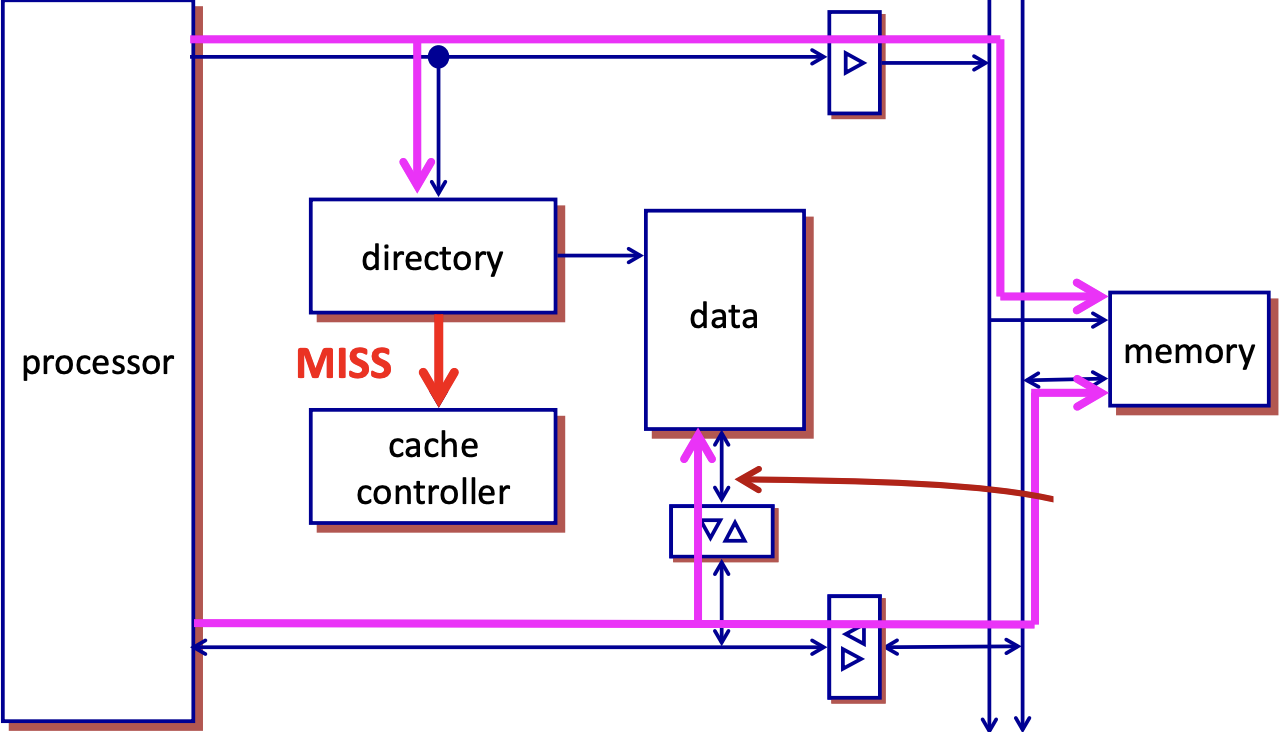
\includegraphics[width=0.65\textwidth]{chapters/chapter3a/images/write_miss.png}
\end{center}
A \textbf{write miss} occurs when the data to be written is not found in the cache. The system must determine how to handle this scenario. The process includes the following steps:

\begin{itemize}
    \item \textbf{Cache Lookup:} The \textit{directory} is checked for the requested address. If the address is not present, a \textbf{miss} signal is sent to the \textit{cache controller}.
    \item \textbf{Memory Update:} The data is written directly to the main memory. This operation ensures that the memory reflects the most recent changes.
    \item \textbf{Cache Allocation:} A decision is made whether to allocate space in the cache for the new data. Two strategies can be employed:
    \begin{enumerate}
        \item \textbf{Write-Allocate:} The data is loaded into the cache after being written to memory, ensuring faster future access.
        \item \textbf{No-Write-Allocate:} The data is written only to the memory, and the cache remains unchanged. This approach reduces cache pollution.
    \end{enumerate}
\end{itemize}

The choice between \textbf{write-allocate} and \textbf{no-write-allocate} is influenced by workload characteristics and system design, balancing cache utilization and memory performance.

\subsubsection{Allocation Policies}

Allocation policies define how data is managed in the cache during a write miss. The two primary policies are:

\paragraph{Write-Allocate:}
\begin{itemize}
    \item On a write miss, the data is also placed in the cache.
    \item This approach is simple and straightforward.
    \item Requires fetching the block of data from memory before writing.
    \item May lead to unnecessary cache pollution if the processor writes data that it will never read back.
\end{itemize}

\paragraph{Write-Around (or Write-No-Allocate):}
\begin{itemize}
    \item On a write miss, the data is written directly to memory, bypassing the cache.
    \item If the processor later loads from the same address, it results in a read miss.
\end{itemize}


\newpage
\section{Summary}
\subsection{The ``3 Cs'' of Caches}

Cache misses are categorized into three types, commonly referred to as the ``3 Cs'':

\paragraph{Compulsory Misses:}
\begin{itemize}
    \item These misses occur during the first reference to a block, even in an infinitely large fully-associative cache.
    \item Also known as \textit{cold-start misses} or \textit{first-reference misses}.
\end{itemize}

\paragraph{Capacity Misses:}
\begin{itemize}
    \item Occur when the cache is unable to hold all the required blocks due to its limited capacity.
    \item These misses happen even in a fully-associative cache.
\end{itemize}

\paragraph{Conflict Misses:}
\begin{itemize}
    \item These occur when multiple blocks compete for the same cache set due to limited associativity.
    \item Arise in set-associative or direct-mapped caches.
\end{itemize}

Understanding these types of misses is critical for identifying the source of limited cache performance.

\subsection{Summary of Cache Features}

This section provides an overview of the key features and attributes of caches:

\begin{itemize}
    \item[-] \textbf{Cache Size:} Total data storage capacity (usually excludes tags, valid bits, dirty bits, etc.).
    \item[-] \textbf{Addressing:} Data can be addressed by byte or word.
    \item[-] \textbf{Line or Block Size:} Specifies the size of cache lines or blocks in bytes or words.
    \item[-] \textbf{Associativity:} Can be fully-associative, $k$-way set-associative, or direct-mapped.
    \item[-] \textbf{Replacement Policy:} Governs how cache blocks are replaced (e.g., LRU, FIFO, random). This is not applicable for direct-mapped caches.
    \item[-] \textbf{Write Policy:} Determines how writes are handled (e.g., write-through or write-back).
    \item[-] \textbf{Allocation Policy:} Defines cache behavior on a write miss (e.g., write-allocate or write-around).
\end{itemize}
\textbf{Cache Addressing}
\begin{center}
    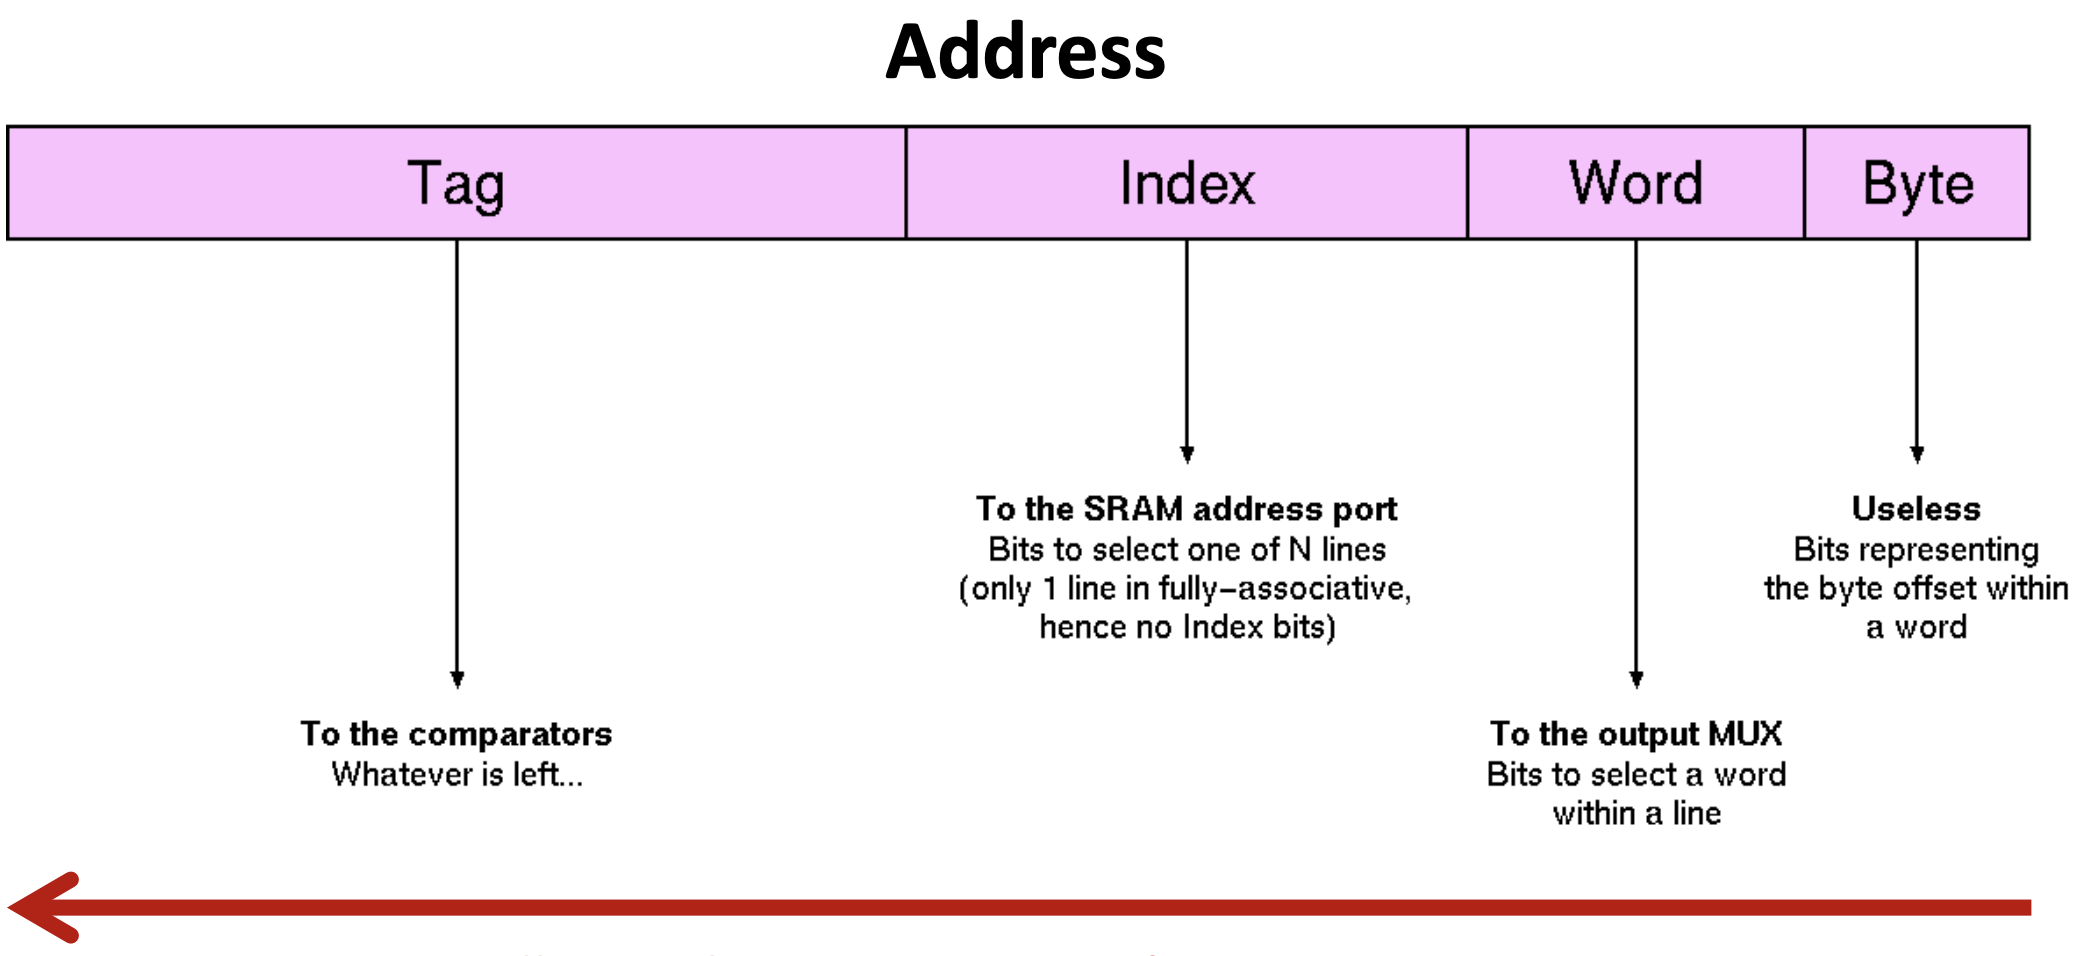
\includegraphics[width=0.75\textwidth]{chapters/chapter3a/images/summary_add.png}
\end{center}
